\documentclass[a4paper,12pt]{article} 
% Paquetes......................................................................
\usepackage{amsmath, amssymb, amsfonts, latexsym}
\usepackage[utf8]{inputenc}
\usepackage[T1]{fontenc}
\usepackage{palatino}
\usepackage[full]{textcomp}
\usepackage{hyperref}
\usepackage{eurosym} % para el simbolo de euro bonito
\usepackage[makeroom]{cancel}
\usepackage{array}
\usepackage{pdfpages}
\usepackage{float} % para que las figuras no floten
\usepackage{subcaption}
\usepackage{soul}
\usepackage{pythonhighlight} % para el entorno python de listings

\textheight = 24 cm
\textwidth = 17 cm

\renewcommand{\arraystretch}{1.25}
\renewcommand{\contentsname}{Contenidos}

% INICIO DEL DOCUMENTO --------------------------------------------------------
\begin{document}
	
	\setlength{\parindent}{0.5cm}
	\setlength{\voffset}{-2cm}
	\setlength{\hoffset}{-2cm}
	
	%%%%%%%%%%%%%%%%%%%%%%%%%%%%%%%%%%%%%%%%%
% Academic Title Page
% LaTeX Template
% Version 2.0 (17/7/17)
%
% This template was downloaded from:
% http://www.LaTeXTemplates.com
%
% Original author:
% WikiBooks (LaTeX - Title Creation) with modifications by:
% Vel (vel@latextemplates.com)
%
% License:
% CC BY-NC-SA 3.0 (http://creativecommons.org/licenses/by-nc-sa/3.0/)
% 
% Instructions for using this template:
% This title page is capable of being compiled as is. This is not useful for 
% including it in another document. To do this, you have two options: 
%
% 1) Copy/paste everything between \begin{document} and \end{document} 
% starting at \begin{titlepage} and paste this into another LaTeX file where you 
% want your title page.
% OR
% 2) Remove everything outside the \begin{titlepage} and \end{titlepage}, rename
% this file and move it to the same directory as the LaTeX file you wish to add it to. 
% Then add \input{./<new filename>.tex} to your LaTeX file where you want your
% title page.
%
%%%%%%%%%%%%%%%%%%%%%%%%%%%%%%%%%%%%%%%%%

%----------------------------------------------------------------------------------------
%	PACKAGES AND OTHER DOCUMENT CONFIGURATIONS
%----------------------------------------------------------------------------------------


%----------------------------------------------------------------------------------------
%	TITLE PAGE
%----------------------------------------------------------------------------------------

\begin{titlepage} % Suppresses displaying the page number on the title page and the subsequent page counts as page 1
	\newcommand{\HRule}{\rule{\linewidth}{0.5mm}} % Defines a new command for horizontal lines, change thickness here
	
	\center % Centre everything on the page
	
	%------------------------------------------------
	%	Headings
	%-----------------------------------------s-------
	
	\textsc{\Large Máster en Inteligencia Artificial}\\[1.5cm] % Main heading such as the name of your university/college
	
	\textsc{\LARGE Métodos de simulación}\\[0.5cm] % Major heading such as course name
	
	%\textsc{\large Minor Heading}\\[0.5cm] % Minor heading such as course title
	
	%------------------------------------------------
	%	Title
	%------------------------------------------------
	
	\HRule\\[0.4cm]
	
	{\huge\bfseries Práctica Grupo 3}\\[0.4cm] % Title of your document
	
	\HRule\\[1.2cm]
	
	%------------------------------------------------
	%	Author(s)
	%------------------------------------------------
	
	%\begin{minipage}{0.4\textwidth}
	%	\begin{flushleft}
	%		\large
	%		\textit{Author}\\
	%		\textsc{Aída Muñoz Monjas} % Your name
	%	\end{flushleft}
	%\end{minipage}
	%~
	%\begin{minipage}{0.4\textwidth}
	%	\begin{flushright}
	%		\large
	%		\textit{Supervisor}\\
	%		Dr. Caroline \textsc{Becker} % Supervisor's name
	%	\end{flushright}
	%\end{minipage}
	
	% If you don't want a supervisor, uncomment the two lines below and comment the code above
	{\Large\textit{Autores}}\\
	
	{\large\textsc{Luis Couto seller\\
			 Irene Marbán Álvarez\\
			 Aída Muñoz Monjas} } % Your name
	
	%------------------------------------------------
	%	Date
	%------------------------------------------------
	
	\vfill\vfill\vfill % Position the date 3/4 down the remaining page
	
	{\large\today} % Date, change the \today to a set date if you want to be precise
	
	%------------------------------------------------
	%	Logo
	%------------------------------------------------
	
	%\vfill\vfill
	%\includegraphics[width=0.2\textwidth]{placeholder.jpg}\\[1cm] % Include a department/university logo - this will require the graphicx package
	 
	%----------------------------------------------------------------------------------------
	
	\vfill % Push the date up 1/4 of the remaining page
	
\end{titlepage}

%----------------------------------------------------------------------------------------

%\end{document}

	
	\tableofcontents
	
\newpage
	\section{Generación de números y variables aleatorias}
	
	\subsection{Enunciado}
	
	Describir el método \textit{Monty Phyton} para la distribución normal y compararlo con otros métodos para la generación de valores de la normal.
	
	\subsection{El método Monty Python}
	
	El objetivo del método Monty Python es lograr generar números aleatorios cuya frecuencia se aproxime a aquella de una distribución normal. Para ello, emplea la similitud entre la expresión de la función de densidad de la distribución normal y una sigmoide decreciente, así como se aprovecha del bajo coste computacional de la generación de números aleatorios en un rectángulo.
	$$ N(0,1) \sim f(x) = \dfrac{1}{\sqrt{2\pi}} \cdot e^{-x^2/2} $$
	
	Tomando $x>0$, se traza un rectángulo de base $b$ y altura $1/b$ sobre la sigmoide. Con un giro de $\pi$ radianes y un desplazamiento sobre la región exterior al rectángulo se pretende representar la mayor superficie posible de la sigmoide en el interior del rectángulo de área $1$. En las imágenes siguientes, podemos observar el procedimiento descrito tomando un $b=2.29$.
	\vspace{-1mm}
	\begin{figure}[H]
		\begin{subfigure}{.5\textwidth}
			\centering
			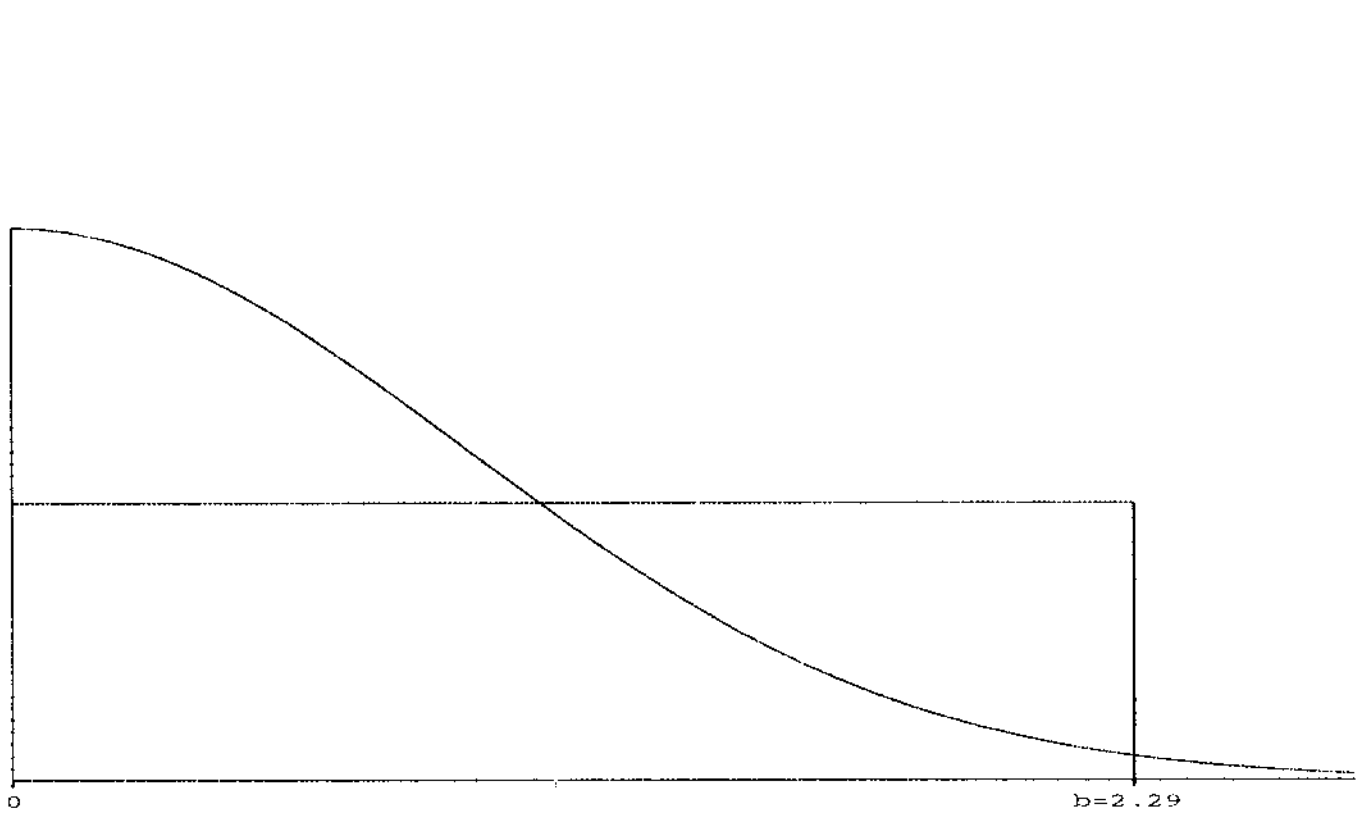
\includegraphics[width=\textwidth]{include/sigmoid_w_square.png}
			\caption{Sigmoide con el rectángulo de base $b$. \cite{monty-python}}
		\end{subfigure}
		\begin{subfigure}{.5\textwidth}
			\centering
			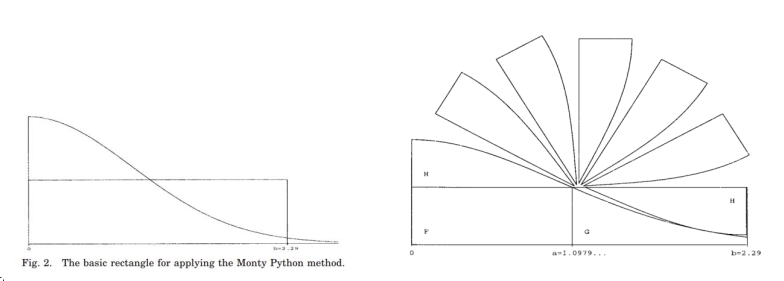
\includegraphics[width=\textwidth]{include/rotating_sigmoid.png}
			\caption{Giro y desplazamiento gráficamente. \cite{monty-python}}
		\end{subfigure}
	\end{figure}
	
	Una vez descrito el área bajo la función de densidad en el interior del rectángulo, todo número aleatorio generado en ese rectángulo pertenecerá a las regiones $F$, $G$, $H$ o a la región comprendida entre $G$ y $H$ correspondiente a la cola de la sigmoide. La probabilidad de obtener un número en la cola es de un $0.022$ \cite{monty-python}.
	
	Siendo $(x,y)$ el valor aleatorio generado, $(x',y')$ será su valor correspondiente en la sigmoide.
	$$
	(x',y') = 
	\begin{cases}
		(x,y) \quad \text{si} \quad x\in F \text{ ó } G \\
		(b-x,2/b-y) \quad \text{si} \quad x \in H
	\end{cases}
	$$  
	
	Si el valor aleatorio generado no pertenece a $F$, $G$ ó $H$, pertenecerá a la cola de la distribución, por lo que basta con devolver una variante de la cola normal mediante el método de Marsaglia o el método de la cola general de Marsaglia y Tsang.\\
		
	La elección del valor de $b$ no es crítica, pero elegir un valor de $b$ demasiado grande implica que habrá solapamiento al realizar el giro y desplazamiento descrito, mientras que si el valor de $b$ es demasiado pequeño, será necesario realizar frecuentemente el método para hallar los valores de la cola.
	En caso de utilizar el método anterior para "ajustar" la sigmoide al rectángulo, la elección de $b=2.29$ es prácticamente la máxima posible \cite{monty-python}. \\
		
	En lugar de una rotación y un desplazamiento de la región exterior al rectángulo, "estirar" la región $H$ permite un ajuste mejor, manteniendo constante el área de la sigmoide, y por tanto siendo este un método más complejo pero más eficiente para realizar dicha aproximación. 
	
	Definiendo el factor de estiramiento $s$ y la función de densidad de la región $H$, $f_H(x)$, 
	$$s=\dfrac{a}{b-a} \hspace{1.5cm} f_H(x)=f(x)-\dfrac{1}{b} \hspace{2mm} \text{con} \hspace{2mm} 0<x<a $$
	se tiene que la región $H$ girada y estirada tiene una función de densidad $f_{H'}(x)$.
	$$ f_{H'}(x) = \dfrac{1}{b} - s  \left[ f(s (b-x) ) -\dfrac{1}{b} \right] $$ 
	La siguiente figura representa gráficamente las transformaciones matemáticas descritas compuestas con la rotación aplicada a la sección $H$. 
	
	\begin{figure}[H]
		\centering
		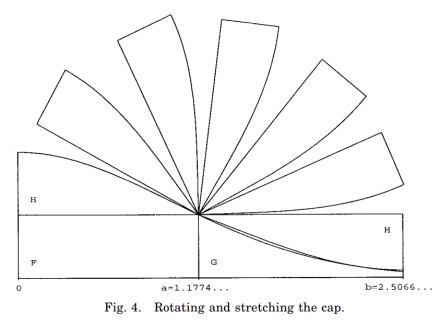
\includegraphics[width=0.6\textwidth]{include/stretching_sigmoid.png}
		\caption{Descripción gráfica del estiramiento descrito. \cite{monty-python}}
	\end{figure}
	
	Para este segundo caso, la elección habitual para el valor de $b$ es $b= \sqrt{2\pi}$. Esta elección no es crítica, cualquier valor entre $2.506$ y $2.5074$ es válido \cite{monty-python}, pero el par $b=\sqrt{2\pi}$, $a = \sqrt{\ln 4}$ son opciones fácilmente identificables con una precisión ilimitada.
	
	
\newpage
	\subsection{Comparación de métodos}
	A continuación, se compararán diferentes métodos para la generación de valores de la normal con el método Monty Python. Para ello, nos basaremos en la publicación citada \cite{comparacion-metodos}. Teniendo en cuenta que tanto el método generador de las secciones $F$, $G$ y $H$, como el método generador de las colas de la sigmoide son relevantes, el artículo divide la evaluación en cuatro secciones.

	
	\begin{itemize}

		\item Tests de bondad de ajuste. Para evaluar los algoritmos utilizados, se utiliza el test $\chi^{2}$. El número de intervalos en los que se divide la distribución para realizar el test es $k$, que se define mediante la siguiente expresión, siendo $n$ el número de muestras.

		\vspace{-5mm}
		$$k = \lceil n^{3/5} \rceil $$
		
		\item Test para valores altos de sigma. Este test mide principalmente el comportamiento de los generadores en las colas de la distribución. El principal reto es la baja probabilidad de obtener muestras que se encuentren en las colas. Se utiliza por tanto un algoritmo para "forzar" la generación de muestras que sean grandes múltiplos de sigma. 

		
		\item Test de aleatoriedad. Para este test, se utiliza la batería Crush, que forma parte de los \textit{TestU01}.

		
		\item Test de correlación interbloque. Este test mide como afecta la distribución de cada una de las muestras a la muestra siguiente, considerándose un buen resultado si la distribución de cada una de las muestras es independiente de las anteriores.

	\end{itemize}

	
	También se evalúa el número de operaciones realizadas y la velocidad de ejecución. 
	
	\subsubsection{Resultados en velocidad.}
	La velocidad se mide relativa a la velocidad del método de Rechazo Polar. El método Monty Python es el cuarto más rápido en comparación con los $16$ otros métodos de generación de variables aleatorias estudiados \cite{comparacion-metodos}, siendo $1.61$ veces más rápido que el método de Rechazo Polar. Cabe destacar que el número de operaciones realizadas es bajo en comparación con el método Wallace, que está por encima del método Monty Python en rapidez. Este último tiene menos cantidad de constantes que el método Ziggurat, que está también por encima del Monty Python en cuestión de velocidad.
	
	\begin{table}[H]
		\centering
		\begin{tabular}{|c||c|}
			\hline
			Nombre del método     & Velocidad     \\ \hline \hline
			Wallace (qual=1)      & 6.41          \\ \hline
			Ziggurat              & 4.29          \\ \hline
			Wallace (qual=4)      & 2.48          \\ \hline
			\textbf{Monty Python} & \textbf{1.61} \\ \hline
			PPND7                 & 1.16          \\ \hline
			Mixture-of-triangles  & 1.14          \\ \hline
			Polar                 & 1.00          \\ \hline   
		\end{tabular}
	\end{table}
	
	\subsubsection{Resultados en el test de bondad de ajuste $\chi^{2}$.}
	En el test de bondad de ajuste $\chi^{2}$, el método Monty Python no pasa el test al utilizar muestras de valores mayores a $2^{34}$. De nuevo, los métodos Wallace y Ziggurat obtienen mejores resultados, ya que no fallan al utilizar muestras de valor igual o mayor a $2^{36}$. El algoritmo PPND7 falla en la misma prueba que el método Monty Python, que a su vez es $3$ veces más lento.
	
	\subsubsection{Resultados en el test de valores altos de sigma.}
	Los resultados de este test muestran el múltiplo más alto de sigma donde el test se realiza con éxito. El método Monty Python obtiene un valor de $8.27$, siendo en este caso mejor que los métodos Ziggurat y Wallace. En comparación con el resto de generadores, el método Monty Python obtiene muy buenos resultados, situándose el cuarto mejor de todos los generadores comparados.
	
	\subsubsection{Resultados del test de aleatoriedad}

	El generador Monty Python no tuvo fallos al realizarse el test Crush.
	
	\subsubsection{Resultados del test de correlación interbloque.}
	Este test solo se realizó en los generadores Ziggurat, Wallace y Monty Pythhon, dado que fueron los más rápidos y en este test se necesitan realizar pruebas con muestras muy grandes. Los generadores de Ziggurat y Monty Python pasaron todos los tests con éxito, mientras que el generador Wallace (tanto el de baja calidad como el de alta), falló con un número inferior a $8$ iteraciones. Esto se debe a que el método Wallace es recursivo.
	
	\subsubsection{Implementación del generador Monty Python}
	Para poder utilizar el generador de Monty Python, una de las opciones mas sencillas es utilizar el packete \texttt{pgnorm} de R, donde esta definido la función \texttt{rpgnorm},
	que permite generar variables siguiendo una normal utilizando Monty Python, Ziggurat, Polar, entre otros. \cite{mp}. \\
	A demás, los propios autores del paper original proporcionan el codigo en C para implementar el algoritmo localmente.

	\subsubsection{Conclusiones}
	Si bien es cierto que el método Wallace es el más rápido, presenta desventajas evidentes como la correlación. \\
 
	El método Ziggurat, que es más lento que el Wallace, no tiene problemas de correlación, pero si que falla en el test Crush con una colisión identificada en los tests de doble precisión. \\
 
	Además, utiliza un total de $388$ constantes, lo que puede ser problemático en algunos entornos. \\
 
	El método Monty Python es el tercero más rápido después del Wallace y el Ziggurat, y presenta ventajas evidentes, como los buenos resultados en los tests de aleatoriedad y correlación, así como el bajo número de operaciones y constantes necesarias. 
	La mayor limitación del método Monty Python está en el uso de muestras cuya $n$ sea mayor que $2^{36}$. 
	
	
	\newpage

	\section{Simulación de sucesos discretos y optimización}

	\subsection{Enunciado}
	Consideremos un almacén de dos productos cuyos precios de venta al público son de $2.5$ y $3.5$ euros la unidad, respectivamente. La llegada de clientes al almacén se distribuye según un proceso de Poisson de parámetro $\lambda = 1.5$ clientes por hora y la cantidad de productos demandados por cada uno de ellos tiene la siguiente distribución:

	\begin{table}[H]
		\centering
		\begin{tabular}{|l||c|c|c|c|}
			\hline
			Demanda    & 1 unidad & 2 unidades & 3 unidades & 4 unidades \\ \hline \hline
			Producto 1 & 0.3      & 0.4        & 0.2        & 0.1        \\ \hline
			Producto 2 & 0.2      & 0.2        & 0.4        & 0.2        \\ \hline
		\end{tabular}
	\end{table}
	
	Para satisfacer la demanda de sus clientes el dueño del almacén mantiene un stock de productos. La política de pedidos al distribuidor es periódica, es decir todos los viernes a primera hora realiza un pedido, tomando como referencia el nivel de inventario de los productos en ese. Para satisfacer la demanda de sus clientes el dueño del almacén mantiene un stock de productos. La política de pedidos al distribuidor es periódica, es decir todos los viernes a primera hora realiza un pedido en el que tomando como referencia el nivel de inventario de los productos en ese momento, se solicitan las unidades necesarias para que el nivel del inventario de cada producto llegue a $1000$ y $1500$ unidades, respectivamente en cada producto.\\

	Asociado a cada pedido que realizamos al proveedor existe un coste fijo (coste de preparación) de $100$ euros, independientemente de las unidades demandadas. Adicionalmente, el coste por unidad incluida en el pedido depende de la cantidad solicitada habiendo descuentos por cantidad. Si el número de unidades demandadas del primer producto es menor o igual a $600$ el precio es de $1$ euro la unidad, mientras que si se piden más de $600$ el precio desciende a $75$ céntimos. Para el segundo producto, si el número de unidades demandadas es menor que $800$ el precio es de $1.5$ euros la unidad, mientras que si se piden más de $800$ el precio desciende a $1.25$ euros.\\

	El tiempo que tarda en ser servido el pedido por los proveedores (tiempo líder), sigue una distribución normal de media 48 horas y desviación típica $3.5$, pagándose en ese momento.\\

	Se ha llegado a un acuerdo con el proveedor de forma que, tomando como referencia las $48$ horas que tarda en media un pedido en ser servido, si el pedido llega con $3$ horas de retraso en la entrega del mismo se realiza un descuento del $0.03\%$ del valor del pedido, encareciéndose en la misma cantidad en el caso de que el pedido llegue con al menos $3$ horas de adelanto.\\
	
	El dueño del almacén debe pagar $0.0002$ euros por unidad del producto y unidad de tiempo, asociado al almacenamiento físico de los productos (alquiler del local, refrigeración...). En el caso de que al llegar un cliente éste solicite una cantidad mayor que la que hay en inventario, se le sirve lo que queda, perdiendo la venta restante.
	
	\begin{enumerate}
		\item[a)] Simular el comportamiento de almacén durante un periodo de tiempo de $5$ meses para estimar el beneficio esperado, la proporción de clientes cuya demanda se satisface completamente y el porcentaje de tiempo que el nivel del inventario permanece a cero. Para ello, supondremos que el nivel del inventario inicial es de $70$ unidades de ambos productos.

		\item[b)] Representar gráficamente la evolución del nivel del inventario durante los $5$ meses y durante los $5$ primeros días. 

		\item[c)] Mediante el uso de la metaheurística recocido simulado identificar cuál será la política de pedidos óptima, es decir, identificar cada cuánto tiempo se deberían realizar los pedidos y el valor de referencia del inventario para identificar el número de unidades a solicitar en la política de pedidos periódica.
	\end{enumerate}
	
	\textbf{Nota.} El almacén permanece abierto las $24$ horas al día de lunes a domingo. El proveedor y la empresa transportista (que sirve los pedidos) también trabajan las $24$ horas, no cerrando en ningún momento.

	\subsection{Modelado del problema}
	El problema descrito se puede representar según el diagrama a continuación.


	\begin{figure}[H]
		\centering
		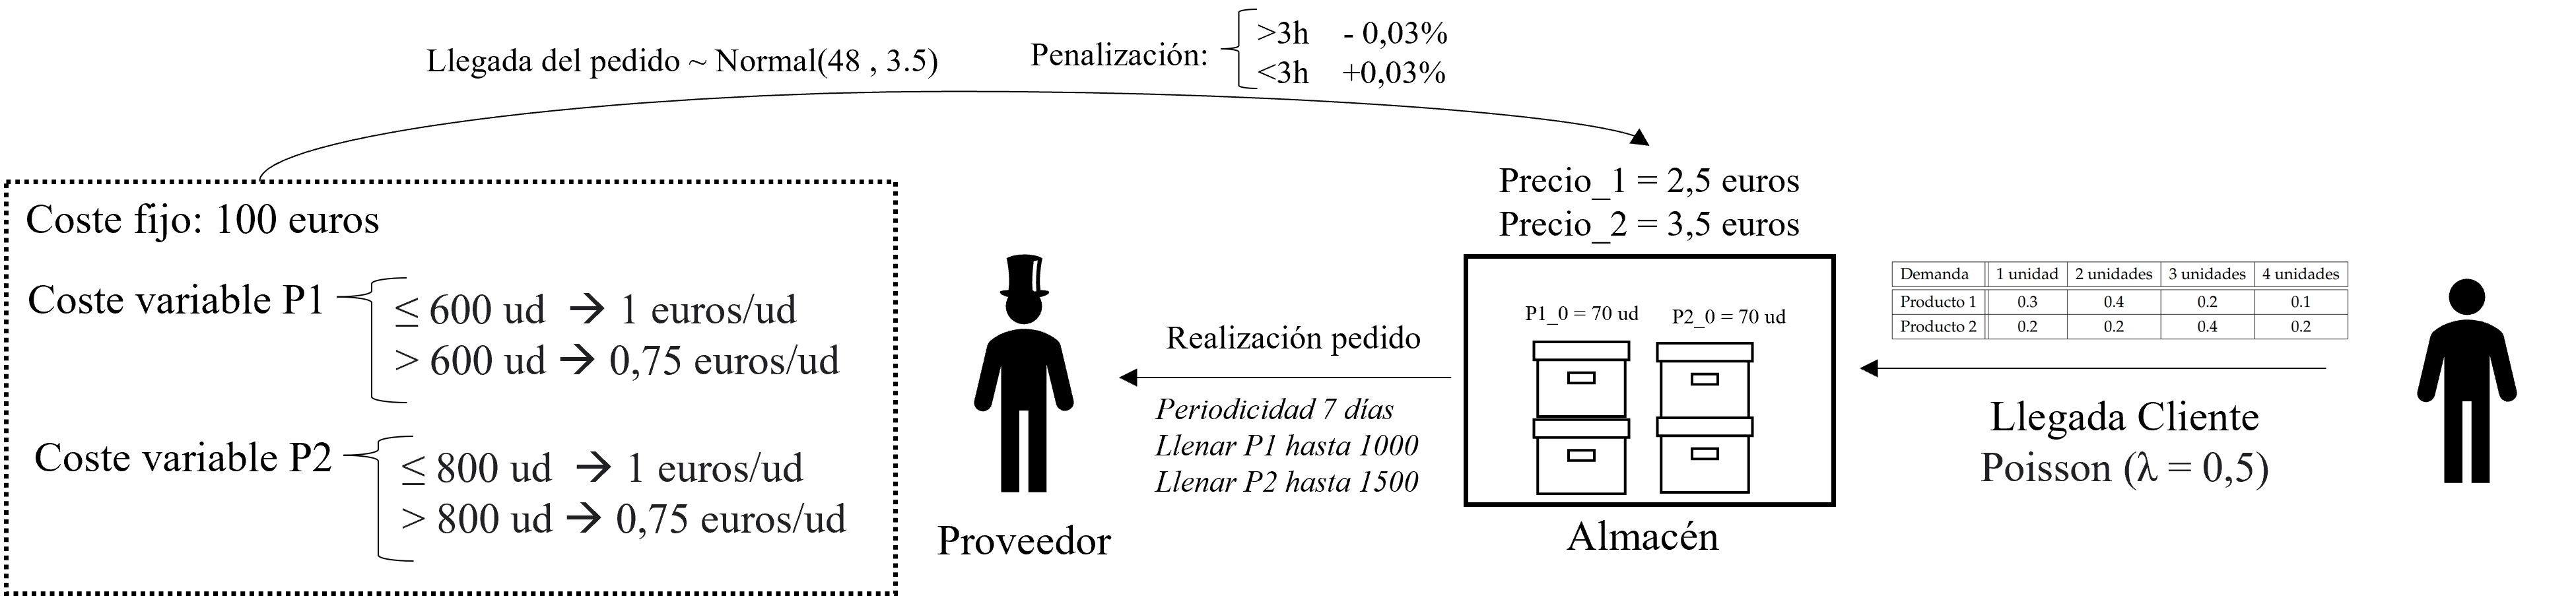
\includegraphics[width=\textwidth]{include/modelo_almacen_v2.png}
		\caption{Representación gráfica del modelado del problema}
	\end{figure}
	
	El almacén guarda productos de dos tipos, siendo $x_1$ y $x_2$ la cantidad de cada uno de los productos almacenados en un instante. Los productos se guardan por separado, teniendo una cantidad máxima de cada producto en stock.\\
	
	Una de las principales características de este problema es su política de pedidos. Cada $7$ días el propietario realiza un pedido al proveedor, independientemente del estado del almacén durante los días anteriores.\\
	
	La llegada de clientes al sistema sigue una distribución de Poission con $\lambda = 0.5$, mientras que la llegada de pedidos sigue una normal $N(48, 3.5)$.\\
	
	El coste total del sistema se calcula como las ganancias por las ventas de productos ($R$) menos los costes de almacenamiento ($H$) y costes de compra de productos al proveedor ($C$).
	
	
	
	\subsection{Simulación del problema. Estimación de beneficios y satisfacción de clientes.}
	Según lo indicado en el apartado a), el objetivo de esta sección es obtener los siguientes valores.
	\begin{itemize}
		\item Estimación el beneficio esperado.
		\item Proporción de clientes cuya demanda se satisface completamente.
		\item Porcentaje de tiempo que el nivel del inventario permanece a cero.
	\end{itemize}
	Se simulará el comportamiento del sistema durante $5$ meses, teniendo inicialmente $70$ unidades de ambos productos en el almacén.
	 	
	\subsubsection{Implementación}
	La implementación de esta simulación se realizó utilizando el lenguaje python, definiendo de manera separada las rutinas de llegada de un cliente, llegada de un pedido y compra de un pedido.\\
	
	Las variables utilizadas se definen como globales, permitiendo que la entrada de cada uno de los métodos sea únicamente el tiempo de simulación (\textit{ts}). No existen problemas de acceso concurrente a las variables, ya que todo el proceso de simulación sucede de manera lineal.
	
	A continuación se destacarán las rutinas utilizadas para cada tipo de evento:
	\begin{itemize}
		\item \textbf{Llegada de un cliente}. 
		
		Esta rutina se ejecuta con la llegada de un nuevo cliente al sistema. Se actualizan los costes de almacenamiento y el estado del almacén, así como los beneficios en caso de poder satisfacer las necesidades del cliente. 
		Cabe resaltar que un cliente no se considera satisfecho si recibe el pedido deseado de uno de los productos, pero no del otro.
		
		En este método se genera también la llegada del siguiente cliente.\\
		
		\begin{python}
def rutina_llegada_cliente(ts):
	global H, h, t_real, x_1, x_2, Nc, Nnc, var_aux, R, Y, y_1, y_2
	global r_1, r_2, var_aux, T_simulacion
	
	#Aumenta el coste de almacenamiento
	H += (ts-t_real)*h*(x_1+x_2)
	t_real = ts

	
	#Generamos demanda del cliente
	demanda_1 = np.random.choice(demanda, 1, p=probab_1)[0]
	demanda_2 = np.random.choice(demanda, 1, p=probab_2)[0]
	
	#Si hay suficiente almacenado, esta satisfecho
	if demanda_1<=x_1 and demanda_2<=x_2 :
		R += demanda_1*r_1 + demanda_2*r_2 #sube el beneficio
		x_1 -= demanda_1	 #baja el inventario
		x_2 -= demanda_2
		Nc += 1 #cliente satisfecho
	#Si no hay suficiente almacenado de algun producto, no esta satisfecho
	else:
		if(demanda_1<=x_1):
			R += demanda_1*r_1
			x_1 -= demanda_1
		elif(demanda_2<=x_2):
			R += demanda_2*r_2
			x_2 -= demanda_2
		Nnc += 1 #cliente no satisfecho
	
	# Si se ha vaciado del todo (y antes no estaba vacio) guardamos cuando
	if x_2 == 0 and x_1 == 0 and var_aux == 0 :
		var_aux = t_real

	
	#Generamos el tiempo que tarda en llegar el siguiente cliente
	Y = stats.poisson.rvs(lambda_poisson, size=1)[0]
	
	# si el cliente llega antes de acabar la simulacion, se simula
	if Y+t_real < T_simulacion:
		lista['tc'] = t_real+Y
		\end{python}
	
	\item \textbf{Llegada de un pedido}. 
	
	Esta rutina se ejecuta con la llegada de un pedido que se compró en el pasado al sistema. Se actualizan los costes de almacenamiento, así como el nivel de inventario posterior a la recogida del pedido. Según el tiempo de llegada del pedido, se calcula el precio de la compra.
	Hemos interpretado que $K$ es el coste fijo de preparar un lote de cada tipo de producto, por lo que se tiene en cuenta para cada uno de los dos tipos de producto producido por separado.\\
	
	\begin{python}
def rutina_llegada_pedido(ts):
	global H, K, h, t_real, C, t0, var_aux, x_1, x_2, y_1, y_2
	global p1_1, p1_2, p2_1, p2_1, penal, var_aux
	
	#Aumenta el coste de almacenamiento
	H += (ts-t_real)*h*(x_1+x_2)
	t_real = ts
	
	#Aumenta el nivel de inventario
	x_1 += y_1
	x_2 += y_2
	
	#Si son muchas unidades, descuento en el precio
	Ci_1 = K + y_1 * p1_1 if y_1<=n_descuent_1 else K + y_1 * p1_2
	Ci_2 = K + y_2 * p2_1 if y_2<=n_descuent_2 else K + y_2 * p2_2
	
	#Si llega pronto es mas caro, si llega tarde, es mas barato
	if L < Lref-lim_penal:
		C += (Ci_1 + Ci_2) * (1 + penal)
	elif L > Lref+lim_penal:
		C += (Ci_1 + Ci_2) * (1 - penal)
	else:
		C += Ci_1 + Ci_2
		
	#Ya no quedan productos por llegar
	y_1 = 0
	y_2 = 0
	
	# Si estaba vacio el inventario (se vacio en el instante var_aux),
	# aumenta el tiempo que ha estado vacio.
	if var_aux > 0:
		t0 += t_real - var_aux
		var_aux = 0
	\end{python}
	
	\item \textbf{Compra de un pedido}. 
	
	Esta rutina se ejecuta en la compra de un nuevo pedido para el almacén. De acuerdo con las indicaciones del enunciado, cada siete días se realiza una compra de la cantidad restante para completar el almacén de cada uno de los productos. \\
	
	\begin{python}
def rutina_compra_pedido(ts):

	global H, x_1, x_2, t_real, y_1, y_2, h, t_real
	global P1, P2, lista, T_simulacion
	
	# Aumenta el coste de almacenamiento
	H += (ts-t_real)*h*(x_1+x_2)
	t_real = ts
	
	#Cantidad a pedir es lo que falta para llenar el almacen
	y_1 = P1 - x_1
	y_2 = P2 - x_2
	
	#Generamos cuanto va a tardar en llegar el pedido
	L = np.random.normal(mu, sigma, 1)[0]
	
	# actualizamos el tiempo de llegada del pedido y el tiempo de siguiente compra
	if L+t_real < T_simulacion:
		lista['tp'] = t_real + L
	
	if t_real+Tp < T_simulacion:
		lista['tpc'] = t_real + Tp
	\end{python}
	
	\end{itemize}
	
	\subsubsection{Resultados y representación gráfica}
	En esta sección se muestran los resultados de la ejecución de la simulación descrita. Tal y como
	se ha descrito en la sección de implementación del código, se ha llevado un seguimiento de la
	simulación gracias a las sentencias \textit{print()} que se han colocado en las distintas funciones del script.
Ejemplos de las salidas para cada uno de los eventos posibles son:
	\begin{itemize}
		\item \textbf{Llegada de un cliente.} Podemos hacer un seguimiento del momento en el que se produce
la llegada del cliente, cuántas unidades demanda de cada producto y el estado del almacén
antes y después del servicio.
		\begin{figure}[H]
			\centering
			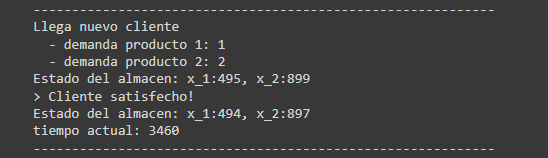
\includegraphics[width=0.75\textwidth]{include/llegada_cliente.png}
		\end{figure}
		
		\item \textbf{Realización de un pedido.} Se muestra el instante de tiempo en el que se realiza el pedido,
el estado del almacén en ese momento y el tiempo que tardará en llegar dicho pedido.
		\begin{figure}[H]
			\centering
			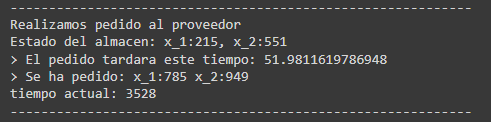
\includegraphics[width=0.75\textwidth]{include/realizacion_pedido.png}
		\end{figure}
	
	
		\item \textbf{Llegada del pedido.} Se indica el instante en el que llega el pedido, el nivel de inventario
 antes y después de la llegada del pedido, y el tiempo que el almacén estuvo vacío en caso
de haber sido así.
		\begin{figure}[H]
			\centering
			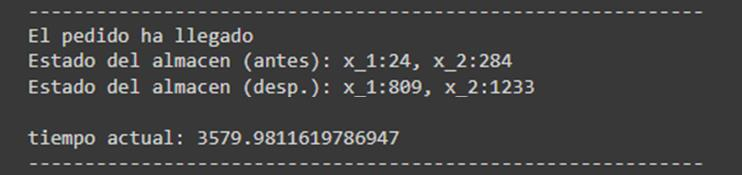
\includegraphics[width=0.75\textwidth]{include/llegada_pedido.png}
		\end{figure}
		
	\end{itemize}

	En la siguiente gráfica podemos ver la evolución de los niveles de inventario de los productos $1$
y $2$ a lo largo del tiempo de simulación ($5$ meses), equivalente a $3600$ horas. Podemos
observar cómo se repite para cada tipo de producto la estructura de picos a lo largo del tiempo
con unas alturas variables pero muy cercanas.
	\begin{figure}[H]
		\centering
		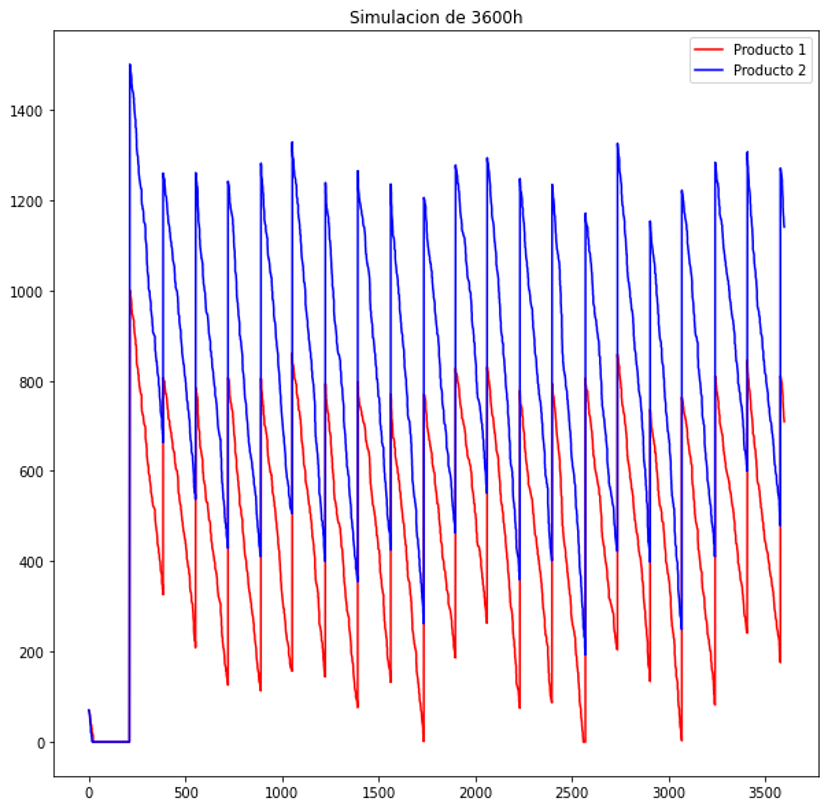
\includegraphics[width=\textwidth]{include/simulacion/simulacion_3600h.png}
	\end{figure}

	\begin{itemize}
		\item Durante el tiempo de simulación el total de ingresos recibidos gracias a las compras de
	los clientes es de $93\hspace{1mm}720$ euros.

		\item En total se han realizado $21$ pedidos que suman un gasto de $39\hspace{1mm}026.20$ euros.

		\item El coste de almacenamiento de los productos ha sido de $904.03$ euros.
	\end{itemize}

	Para calcular el beneficio obtenido basta con restar a los ingresos los gastos de pedido y los gastos
de almacenamiento:

	$$beneficio = 93\hspace{1mm}720 - 39\hspace{1mm}026.20 - 904.03 = 53\hspace{1mm}789.76$$
	
	
	Partiendo de un nivel de inventario de $70$ unidades de cada tipo de producto, y con la política de
pedidos descrita en el enunciado, la proporción de tiempo que el almacén está completamente
vacío es de un $5.25\%$ del tiempo, lo que en horas equivale a $189$ horas.

	
	En $3\hspace{1mm}600$ horas han llegado un total de $7\hspace{1mm}298$ clientes de los cuales:
	
	\begin{itemize}
		\item $6\hspace{1mm}497$ clientes su demanda ha sido completamente satisfecha.
		\item $400$ clientes su demanda no ha sido satisfecha.
	\end{itemize}

	Eso supone que la demanda de un $94.20\%$ de los clientes que llegaron a la tienda en este periodo

	de $5$ meses fue totalmente satisfecha.
	
	Analizando los resultados, si observamos más de cerca en la gráfica el periodo de tiempo que
comprende los $5$ primeros días de la simulación ($120$ horas), podemos observar que debido al
nivel inicial de inventario y a que la política de pedidos establece que los pedidos se hacen de
forma periódica cada $168$ horas (cada $7$ días), hay una gran franja en la que el inventario de ambos
productos está a $0$ sin poder satisfacerse la demanda de los clientes que llegan en ese periodo.
	
	\begin{figure}[H]
		\centering
		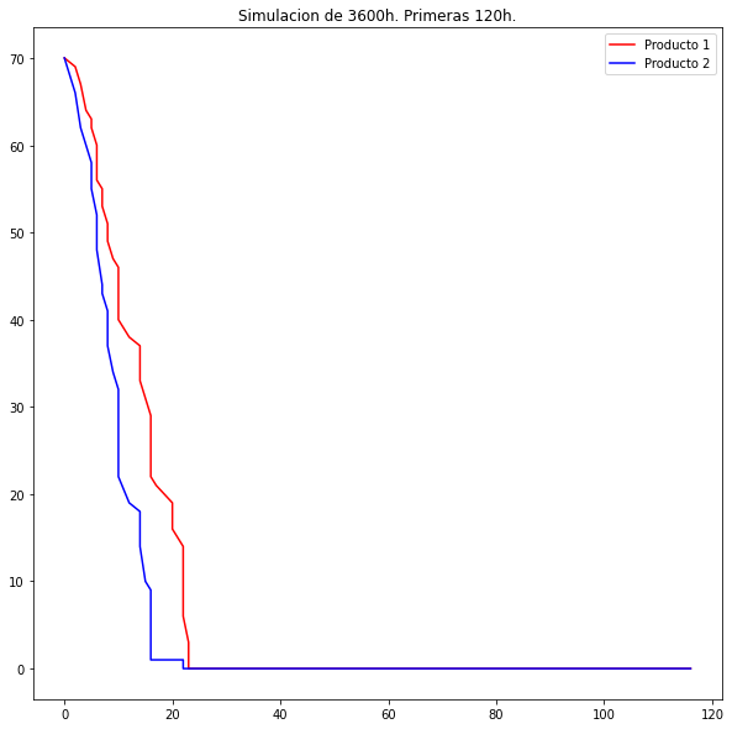
\includegraphics[width=0.75\textwidth]{include/simulacion/simulacion_120h.png}
	\end{figure}
	
	Como se observa, partiendo únicamente con $70$ unidades de cada producto, alrededor de las $22$ 	horas se agotaron las unidades del producto $2$ y a las $24$ horas de simulación ya se habían acabado las existencias de ambos productos quedando completamente vacío el inventario, teniendo que	esperar a que se realizara el pedido y a que este llegara.

	\subsection{Simulación del problema con metaheurísticas. Identificación de política de pedidos óptima.}
	
	\subsubsection{Introducción al Recocido Simulado}
	
	Debido a la complejidad de los problemas de optimización que se busca resolver en el mundo, la búsqueda local y los métodos clásicos de optimización no son suficientes para modelizar correctamente el gran número de factores de decisión y restricciones que intervienen. Por esta razón se desarrollan las metaheurísticas, dando un paso más allá de las heurísticas clásicas que se centran únicamente en un tipo de problema y pueden quedarse atrapadas en un mínimo local.\\
	
	Las metaheurísticas	utilizan conocimiento de distintas áreas de la ciencia, como puede ser la inteligencia artificial, la estadística, la genética, etc. para proponer algoritmos que generen una solución eficiente  satisfactoria a un problema de optimización.\\
	
	En esta práctica, se nos ha propuesto utilizar una metaheurística de búsqueda global, conocida como \textit{recocido simulado}. Esta metaheurística se basa en el fenómeno de enfriamiento de los metales estudiada en el ámbito de la metalurgia. \\
	
	Para aplicar esta idea a un problema de optimización, se plantean tres etapas:
	\begin{itemize}
		\item En la primera etapa, las soluciones elegidas en el entorno $E(x)$ de manera aleatoria no son necesariamente óptimas. Si la solución generada es mejor que la anterior, la exploramos directamente, pero si es peor, podemos explorarla según una probabilidad determinada por una variable aleatoria. En esta primera fase, la probabilidad de elegir soluciones peores es más alta, evitando así caer en mínimos locales y permitiendo explorar un entorno más amplio.
		\item En la segunda etapa, la probabilidad de que se elija una solución peor ya no es tan alta, pero aún así hay posibilidad de volver atrás.
		\item En la última etapa, sólo aceptaremos movimientos que mejoren la solución actual.
	\end{itemize}
	
	En este algoritmo es muy importante la elección del parámetro \textit{Temperatura}. Este parámetro, ira decreciendo cada $L$ iteraciones, hasta llegar a una temperatura final u otro punto de parada que se haya especificado. La forma en la que la temperatura influye en la búsqueda del algoritmo es mediante la expresión que define la distribución de Boltzman. 
	$$p(i)=e^{-\dfrac{f(y)-f(x_i)}{T_i}}$$
	Esta es la distribución que va a tomar la probabilidad de elegir una solución peor, de manera que si la temperatura es muy alta, la probabilidad de que se elija una solución peor será mayor. La temperatura decrece según la expresión
	$$T_{hL}=\alpha ^h T_1$$
	El valor alfa ($\alpha$) determinará cuanto disminuye la temperatura.
	
	En general, los hiperparámetros que hay que controlar para la ejecución del algoritmo son los siguientes:
	\begin{itemize}
		\item Temperatura inicial
		\item $L$, número de iteraciones que deben pasar para actualizar la temperatura
		\item $\alpha$, velocidad de disminución de la temperatura
		\item Criterio de parada
		\item Entorno para elegir una solución vecina
	\end{itemize}
	
	El problema que buscamos resolver en esta práctica con este algoritmo es encontrar el valor de periodicidad con el que se deben realizar los pedidos, así como la cantidad que se debe pedir de cada uno de los productos para maximizar el beneficio.
	
	\subsubsection{Ajuste de los hiperparámetros}

	\paragraph{Entorno de vecindad}.\\	
	
	
	Como se ha definido previamente, los tres factores de decisión que vamos a ir variando para encontrar un beneficio máximo son: nivel de producto 1, nivel de producto 2 y periodo de pedido. \\
	Nuestra implementacion comenzará con un estado inicial donde estos tres parametros toman el valor inicial propuesto para la simulación. Estos valores irán cambiando segun nos movamos a soluciones vecinas, con el último objetivo de 
	encontrar una solción óptima. 
	Para encontrar los niveles de producto de las soluciones vecinas, hemos definido un entorno tamaño 3, de forma que se van a restar o sumar entre 3 y 0 unidades de producto al estado actual. Se utilizará una función 
	independiente para cada producto, de forma que el nivel de producto 1 podria aumentar 3 unidades mientras que el nivel de producto 2 podria disminuir. 
	Para hallar la periodicidad de pedido, que es el otro factor de decisión, en este caso utilizamos una distribución uniforme entre -1 y 1, ya que al tratarse de tiempo puede tomar valores continuos. \\
	Hemos optado por un entorno relativamente pequeño para evitar saltos grandes entre las soluciones, ya que dificultaría la convergencia del algoritmo. 
	
	\paragraph{Temperatura inicial}.\\
	La temperatura inicial que se escoja para la ejecución del algoritmo de recocido simulado presenta una vital importancia para el correcto funcionamiento de esta metaheurística y para la obtención del máximo global buscado.\\

	\begin{figure}[H]
		\centering
		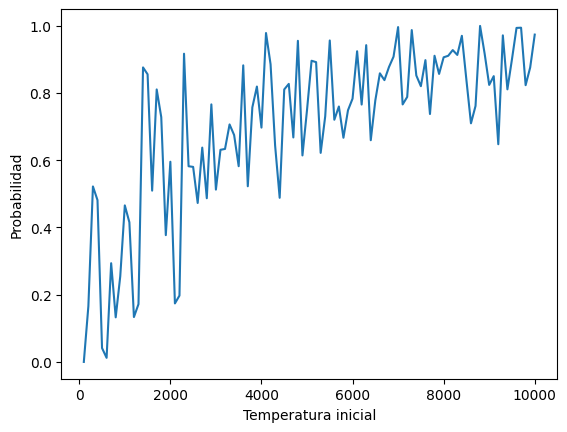
\includegraphics[width=0.75\textwidth]{include/Temperaturas/grafico1.png}
	\end{figure}

	Lo ideal a la hora de elegir la temperatura inicial es escoger aquella que inicialmente proporcione una probabilidad inicial de escoger una solución peor cercana a 0.9. Por ello para explorar el espacio de probabilidades se ha implementado una función que ejecuta la simulación diseñada y calcula la probabilidad con los distintos valores de la temperatura. 

	En la gráfica podemos observar como varía la probabilidad inicial con el cambio de temperatura inicial. Se trata de una probabilidad que fluctúa mucho ya que esta depende de muchos elecciones aleatorias realizadas tanto en la simulación como en la elección de la solución vecina en el entorno de la solución inicial. Aun siendo muy variable se observa como hay una tendencia creciente que se estabiliza ligeramente cuando llegamos hacia el rango de temperatura entre 7000 y 8000. Es por ello por lo que decidimos volver a ejecutar la búsqueda de la temperatura inicial pero en ese rango para observarlo más de cerca:
	
	\begin{figure}[H]
		\centering
		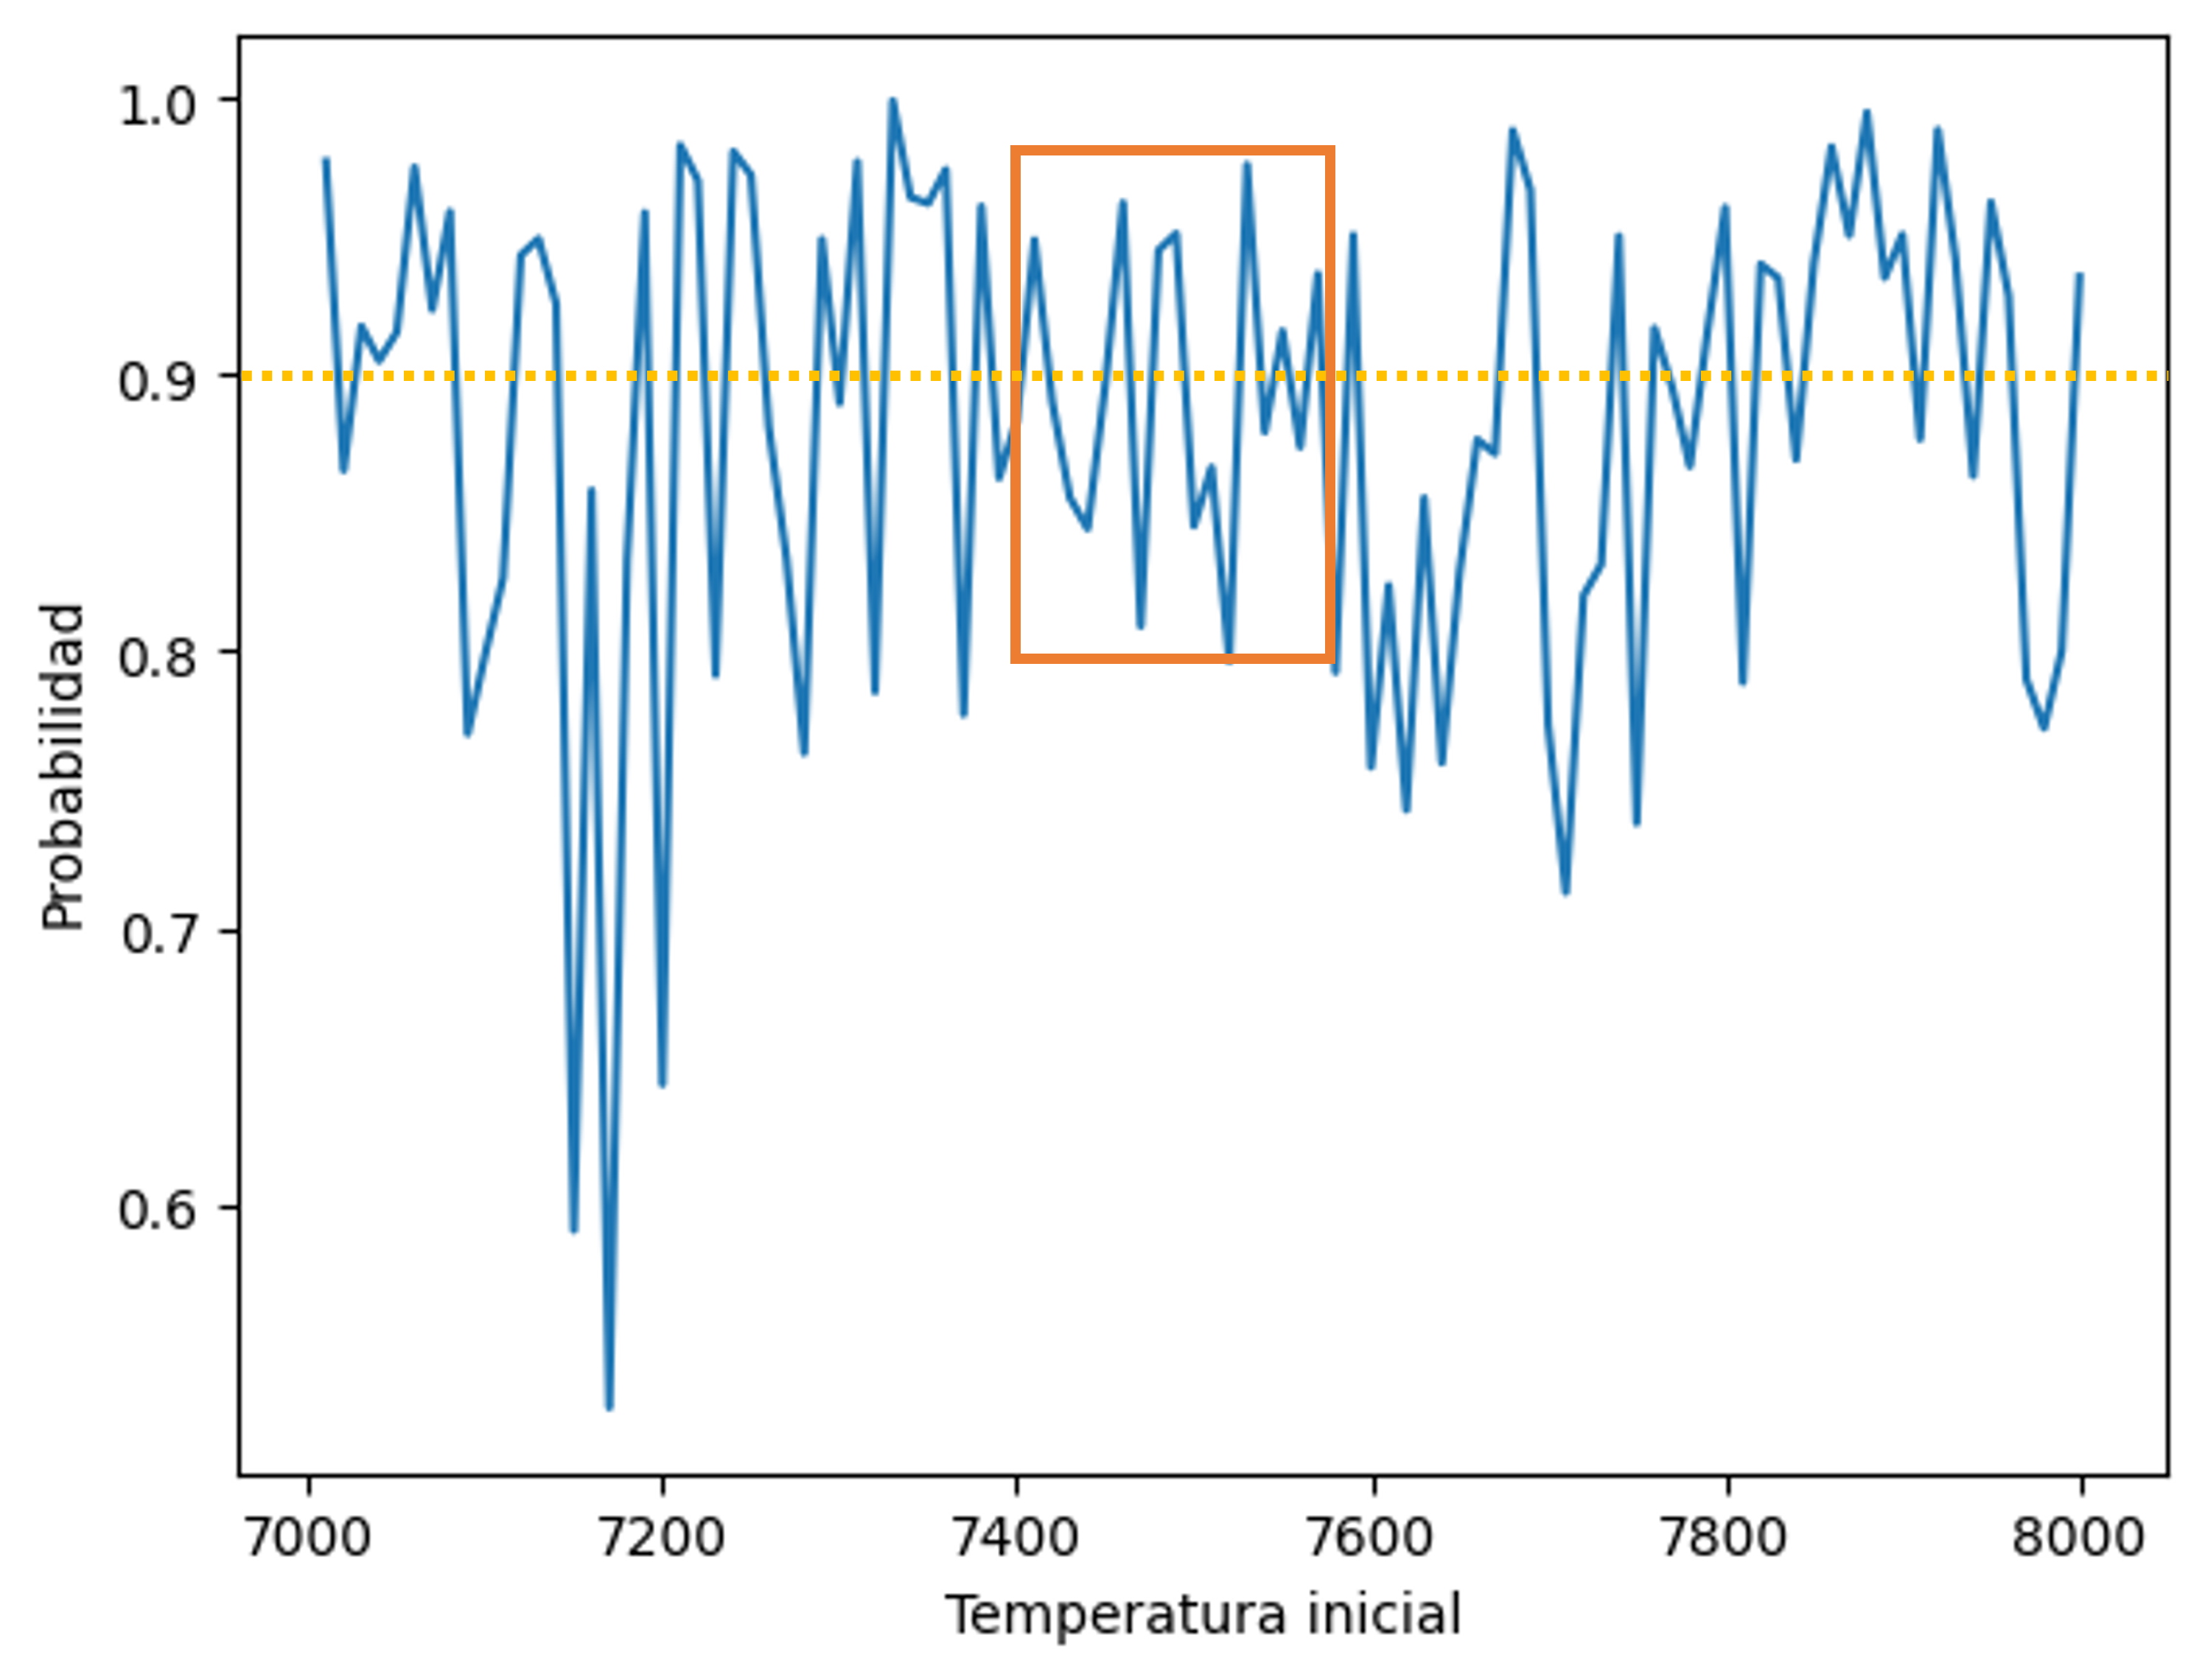
\includegraphics[width=0.75\textwidth]{include/Temperaturas/grafico2.png}
	
	\end{figure}
	Como se observa, aunque las fluctuaciones están un poco más acotadas para estos valores de temperatura, siguen variando bastante, pero hemos podido observar que la franja de temperatura señalada con el recuadro naranja en la anterior gráfica parece un poco más estable y estar en torno a 0.9 de probabilidad.  Por ello se ha escogido el valor de 7500 como temperatura inicial para la ejecución del recocido simulado.\\

	De todas maneras, cabe destacar la dificultad de la correcta elección de la temperatura, se comprobará de manera empírica si efectivamente esta temperatura es adecuada o no para la búsqueda del óptimo global.

	\paragraph{Parámetro L}.\\
	El parámetro L establecerá el número de iteraciones en las que cada temperatura se mantendrá sin variar. Es importante también elegir valor adecuado ya que si escogemos una L muy baja no daremos tiempo al algoritmo para que pueda explorar soluciones peores.\\

	Para explorar las posibilidades, hemos decidido realizar unas pruebas piloto con distintos valores de L y observar la evolución de las soluciones para cada caso. De esta manera podemos ver cual de los valores de L probados es el óptimo, es decir, que no sea muy pequeño y permitir a cada una de las temperaturas quedarse estable el suficiente tiempo como para que explore soluciones peores, pero no sea muy grande para no hacerlo tan ineficiente explorando de manera que no se llega a una solución mejor.\\

	Para estas simulaciones piloto todavía no hemos definido el criterio de parada adecuado, eso se explicará en los siguientes apartados. Para este apartado el criterio de parada que se establece es que el algoritmo para cuando la temperatura llega a un valor de 1, de tal manera que viésemos todo el recorrido del recocido simulado.\\

	Los valores de L con los que hemos hecho pruebas piloto han sido 1, 2, 5 y 10. A continuación se muestran algunos de los resultados más representativos obtenidos tras múltiples pruebas con cada uno de ellos.\\

	
	
	\begin{figure}[H]
		\centering
		\begin{subfigure}{0.24\textwidth}
			\centering
			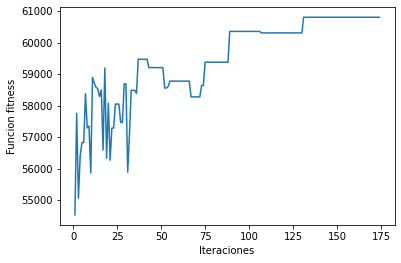
\includegraphics[width=\textwidth]{include/L1/fitness.png}
			\caption{Fitness}
		\end{subfigure}
		\hfill
		\begin{subfigure}{0.24\textwidth}
			\centering
			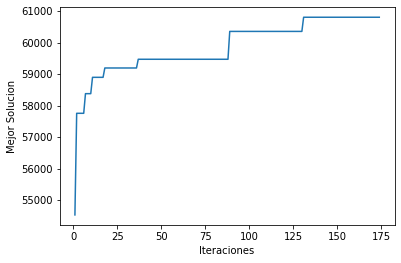
\includegraphics[width=\textwidth]{include/L1/mejor_solucion.png}
			\caption{Mejor solución}
		\end{subfigure}
		\hfill
		\begin{subfigure}{0.24\textwidth}
			\centering
			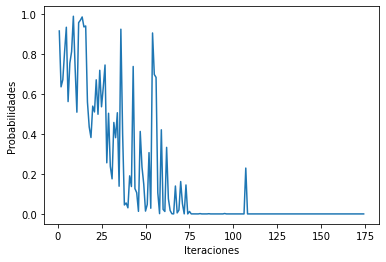
\includegraphics[width=\textwidth]{include/L1/probabilidades.png}
			\caption{probabilidad}
		\end{subfigure}
		\hfill
		\begin{subfigure}{0.24\textwidth}
			\centering
			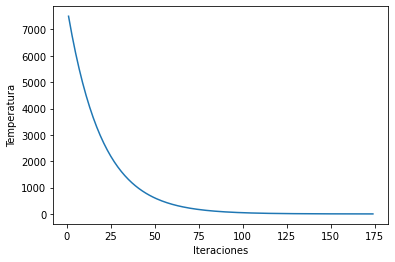
\includegraphics[width=\textwidth]{include/L1/temperatura.png}
			\caption{Temperatura}
		\end{subfigure}
		\caption{Pruebas para L=1. Mejor solución: Periodicidad: 177.62, nivel\_1: 977, nivel\_2: 1519, \textbf{beneficio}: 60806.31. Tiempo de ejecución 3 min 9 s }
	\end{figure}

	\begin{figure}[H]
		\centering
		\begin{subfigure}{0.24\textwidth}
			\centering
			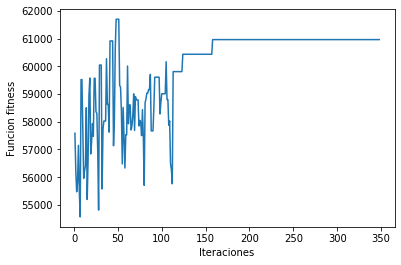
\includegraphics[width=\textwidth]{include/L2/fitness.png}
			\caption{Fitness}
		\end{subfigure}
		\hfill
		\begin{subfigure}{0.24\textwidth}
			\centering
			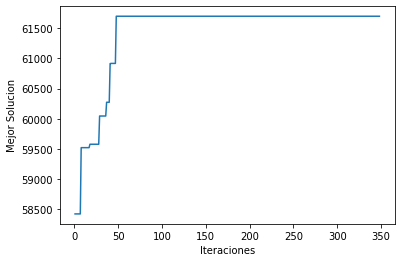
\includegraphics[width=\textwidth]{include/L2/mejor_solucion.png}
			\caption{Mejor solución}
		\end{subfigure}
		\hfill
		\begin{subfigure}{0.24\textwidth}
			\centering
			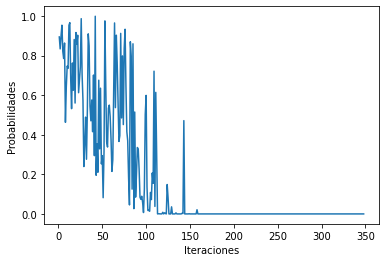
\includegraphics[width=\textwidth]{include/L2/probabilidades.png}
			\caption{probabilidad}
		\end{subfigure}
		\hfill
		\begin{subfigure}{0.24\textwidth}
			\centering
			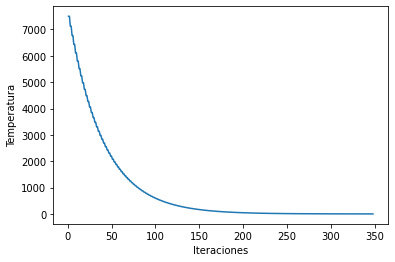
\includegraphics[width=\textwidth]{include/L2/temperatura.png}
			\caption{Temperatura}
		\end{subfigure}
		\caption{Pruebas para L=2. Mejor solución: Periodicidad: 170.27, nivel\_1: 997,  nivel\_2: 1515, \textbf{beneficio}: 61697.25. Tiempo de ejecución 6 min 17 s}
	\end{figure}

	
	\begin{figure}[H]
		\centering
		\begin{subfigure}{0.24\textwidth}
			\centering
			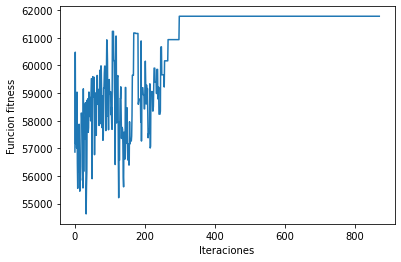
\includegraphics[width=\textwidth]{include/L5/fitness.png}
			\caption{Fitness}
		\end{subfigure}
		\hfill
		\begin{subfigure}{0.24\textwidth}
			\centering
			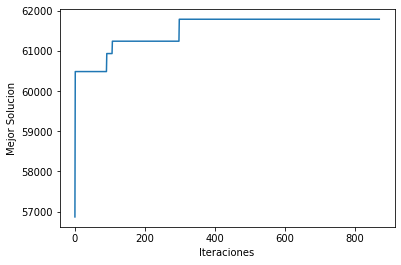
\includegraphics[width=\textwidth]{include/L5/mejor_solucion.png}
			\caption{Mejor solución}
		\end{subfigure}
		\hfill
		\begin{subfigure}{0.24\textwidth}
			\centering
			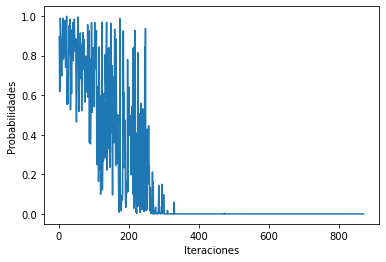
\includegraphics[width=\textwidth]{include/L5/probabilidades.png}
			\caption{probabilidad}
		\end{subfigure}
		\hfill
		\begin{subfigure}{0.24\textwidth}
			\centering
			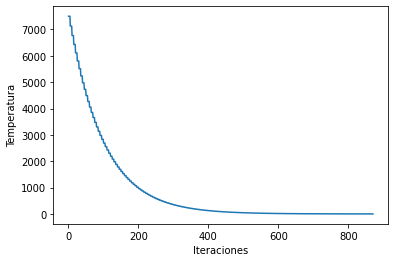
\includegraphics[width=\textwidth]{include/L5/temperatura.png}
			\caption{Temperatura}
		\end{subfigure}
		\caption{Pruebas para L=5. Mejor solución: Periodicidad: 171.26, nivel\_1: 982,  nivel\_2: 1449,\textbf{beneficio}: 61784.29. Tiempo de ejecución 15 min 39 s}
	\end{figure}

	\begin{figure}[H]
		\centering
		\begin{subfigure}{0.24\textwidth}
			\centering
			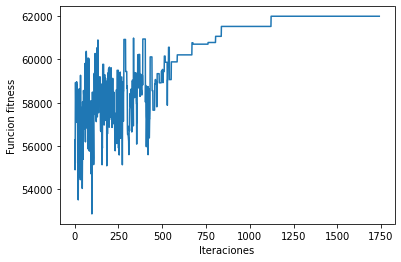
\includegraphics[width=\textwidth]{include/L10/fitness.png}
			\caption{Fitness}
		\end{subfigure}
		\hfill
		\begin{subfigure}{0.24\textwidth}
			\centering
			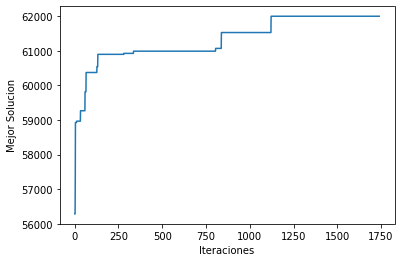
\includegraphics[width=\textwidth]{include/L10/mejor_solucion.png}
			\caption{Mejor solución}
		\end{subfigure}
		\hfill
		\begin{subfigure}{0.24\textwidth}
			\centering
			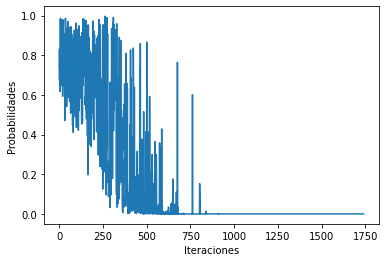
\includegraphics[width=\textwidth]{include/L10/probabilidades.png}
			\caption{probabilidad}
		\end{subfigure}
		\hfill
		\begin{subfigure}{0.24\textwidth}
			\centering
			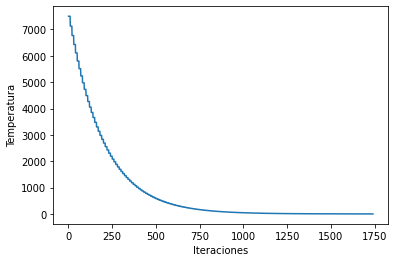
\includegraphics[width=\textwidth]{include/L10/temperatura.png}
			\caption{Temperatura}
		\end{subfigure}
		\caption{Pruebas para L=10. Periodicidad: 161.69, nivel\_1: 938,  nivel\_2: 1530, \textbf{beneficio}: 62001.13. Tiempo de ejecución 31 min 31 s}
	\end{figure}


	
	Como se puede observar, el comportamiento del recocido simulado es similar para todos los valores de L, pero lo que cambia al fin y al cabo es el número de iteraciones que permanecemos en cada temperatura. La diferencia de las mejores soluciones encontradas en cada caso no es muy grande pero si que cabe destacar que para L=10 gracias a que permanece un gran número de iteraciones explorando soluciones peores debido a las altas temperaturas, finalmente consigue llegar a un resultado mayor no visto en las pruebas con Ls más pequeñas.\\

	Como ya se ha mencionado con la temperatura, al tratarse de la optimización de una simulación que tiene una componente aleatoria bastante grande y que puede variar mucho de una ejecución a otra, la elección de L puede ser importante para asegurar que se le da bastantes oportunidades al algoritmo de encontrar soluciones y realizar así bastantes iteraciones. A la vista de los resultados hemos podido comprobar que las pruebas realizadas con una L grande exploraban muchas soluciones y en muchas de las ejecuciones realizadas se alcanzaba un resultado mejor que para L pequeña. Una L pequeña también puede alcanzar un buen resultado, pero debido aque la temperatura alcanza valores bajos de manera más rápida puede variar mucho de una ejecución del recocido a otra y en muchas de estas ejecuciones no alcanzaba un buen resultado, como se ve por ejemplo en L=1 que se queda en el máximo de 60806 euros de beneficio.

	\paragraph{Criterio de parada}.\\
	El criterio utilizado en este recocido simulado como condición de parada es haber alcanzado un número $x$ de iteraciones sin cambios, es decir, que tras $x$ iteraciones seguidas en las que no se ha mejorado la función objetivo, en este caso los beneficios, la simulación debe parar.\\
		
	Para encontrar el valor óptimo de este parámetro se ejecutaron varias pruebas piloto fijando el resto de parámetros indicados en esta sección. Los valores fueron $\alpha = 0.95$, temp. inicial $=7500$, L $=10$, distancia de la búsqueda de nivel del inventario $3$ y distancia de la búsqueda de periodicidad $1$. \\ 
	
	En primer lugar, se usó un valor de $50$, con el que la temperatura no bajó de $5000$ y la solución apenas mejoró, obteniendo un beneficio de $61414.08$\euro \hspace{1mm} al realizar los pedidos con una periodicidad de $172.78$ días y un nivel máximo de producto $1031$ y $1508$ respectivamente.
	%{'periodicidad': 172.77635806601137, 'nivel_1': 1031, 'nivel_2': 1508, 'benef': 61414.08057727425}
	
	Para intentar mejorar los resultados, se aumentó a un valor de $100$, con el que la temperatura aún no bajó de $4000$. En este caso se obtuvo un beneficio de $61537.94$\euro \hspace{1mm} al realizar los pedidos con una periodicidad de $161.65$ días y un nivel máximo de producto $1005$ y $1480$ respectivamente.\\
	%{'periodicidad': 161.65371542849738, 'nivel_1': 1005, 'nivel_2': 1480, 'benef': 61537.93718629534}
	
	Como el valor aún no era suficientemente alto como para que la temperatura bajase a valores cercanos a cero, se usó un valor de $300$. En este caso, la temperatura decrece hasta valores muy cercanos a $0$, y en la gráfica de la solución evaluada se observa la evolución esperada, pasando de una gran variabilidad a una solución óptima más estable. Para esta ejecución se obtuvo un beneficio de $61985.74$\euro \hspace{1mm} al realizar los pedidos con una periodicidad de $170.90$ días y un nivel máximo de producto $938$ y $1467$ respectivamente.\\
	%{'periodicidad': 170.89754956500875, 'nivel_1': 938, 'nivel_2': 1467, 'benef': 61985.738664631484}
	
	La última ejecución piloto usó un valor de $200$, intentando disminuir el tiempo de ejecución manteniendo la calidad de los resultados obtenidos con la ejecución anterior. En este caso, la simulación no llegó a lograr una temperatura suficientemente baja como para lograr un estado en el que los movimientos a estados cercanos sean muy limitados, generando una gráfica de la función fitness diferente a la esperada con esta metaheurística. Se obtuvo un beneficio de $61142.38$\euro \hspace{1mm} al realizar los pedidos con una periodicidad de $169.96$ días y un nivel máximo de producto $993$ y $1523$ respectivamente.\\
	%{'periodicidad': 169.9591639589791, 'nivel_1': 993, 'nivel_2': 1523, 'benef': 61142.376675656706}
	
	Se decidió no aumentar este valor por encima de $300$ ya que la temperatura alcanza valores muy cercanos a $0$ y la probabilidad de moverse a soluciones peores también es muy cercana a $0$, por lo que sería dificil mejorar el rendimiento de este algoritmo con este parámetro.\\
	
	En las siguientes figuras se encuentran las gráficas generadas en cada iteración de la simulación, en las que se pueden apreciar los detalles señalados.
	
	\begin{figure}[H]
		\centering
		\begin{subfigure}{0.24\textwidth}
			\centering
			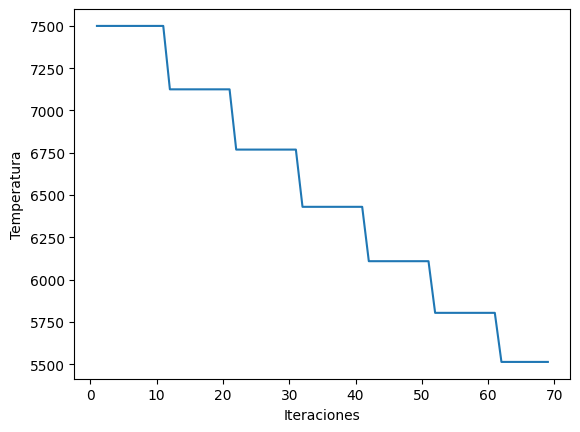
\includegraphics[width=\textwidth]{include/parada/50/temp.png}
			\caption{valor: $50$}
		\end{subfigure}
		\hfill
		\begin{subfigure}{0.24\textwidth}
			\centering
			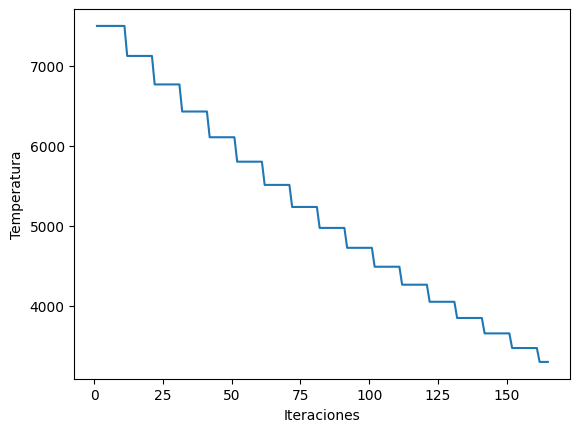
\includegraphics[width=\textwidth]{include/parada/100/temp.png}
			\caption{valor: $100$}
		\end{subfigure}
		\hfill
		\begin{subfigure}{0.24\textwidth}
			\centering
			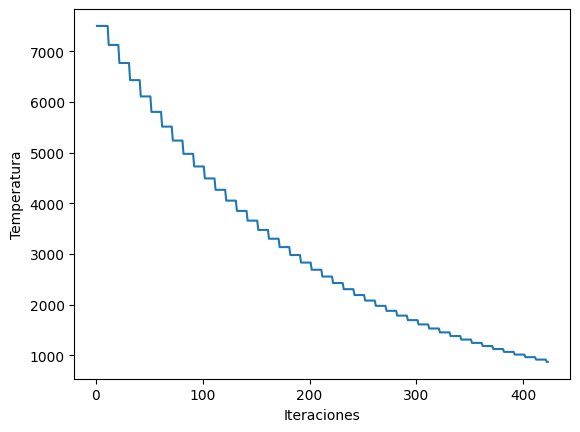
\includegraphics[width=\textwidth]{include/parada/200/temp.png}
			\caption{valor: $200$}
		\end{subfigure}
		\hfill
		\begin{subfigure}{0.24\textwidth}
			\centering
			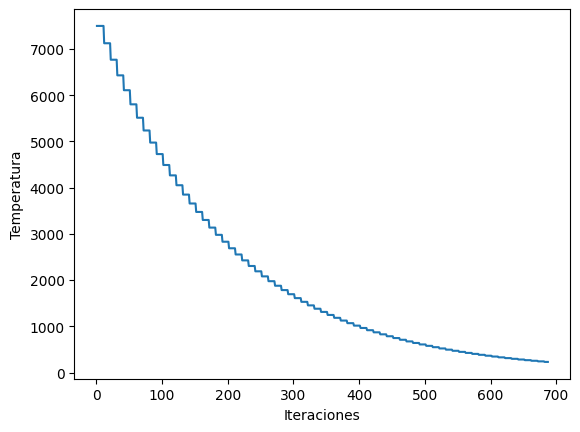
\includegraphics[width=\textwidth]{include/parada/300/temp.png}
			\caption{valor: $300$}
		\end{subfigure}
		\caption{Pruebas para el criterio de parada. Evolución de la temperatura.}
	\end{figure}
	
	\begin{figure}[H]
		\centering
		\begin{subfigure}{0.24\textwidth}
			\centering
			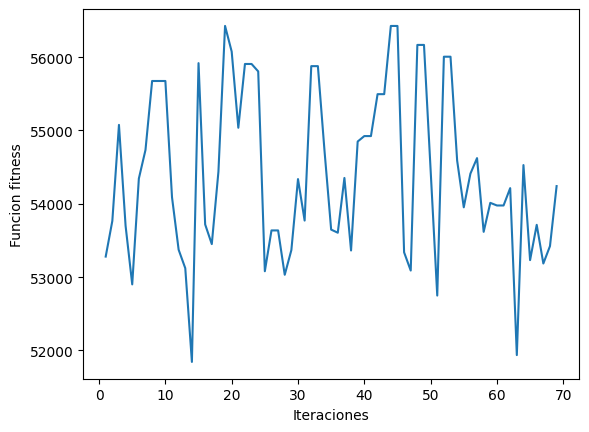
\includegraphics[width=\textwidth]{include/parada/50/f.png}
			\caption{valor: $50$}
		\end{subfigure}
		\hfill
		\begin{subfigure}{0.24\textwidth}
			\centering
			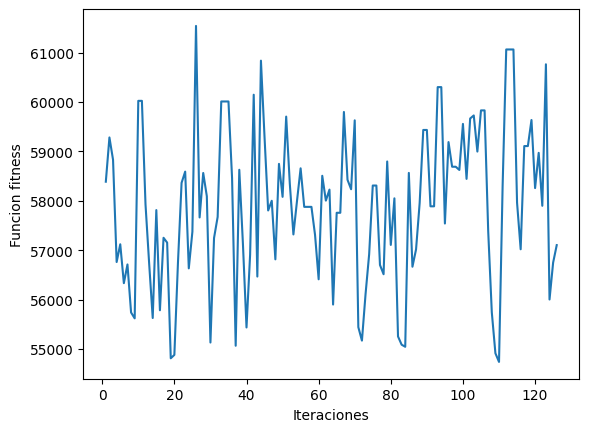
\includegraphics[width=\textwidth]{include/parada/100/f.png}
			\caption{valor: $100$}
		\end{subfigure}
		\hfill
		\begin{subfigure}{0.24\textwidth}
			\centering
			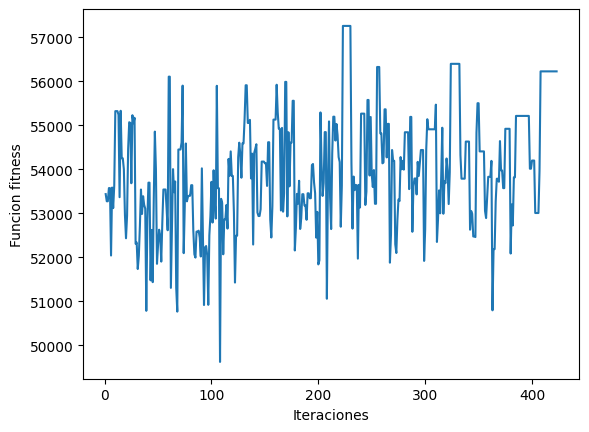
\includegraphics[width=\textwidth]{include/parada/200/f.png}
			\caption{valor: $200$}
		\end{subfigure}
		\hfill
		\begin{subfigure}{0.24\textwidth}
			\centering
			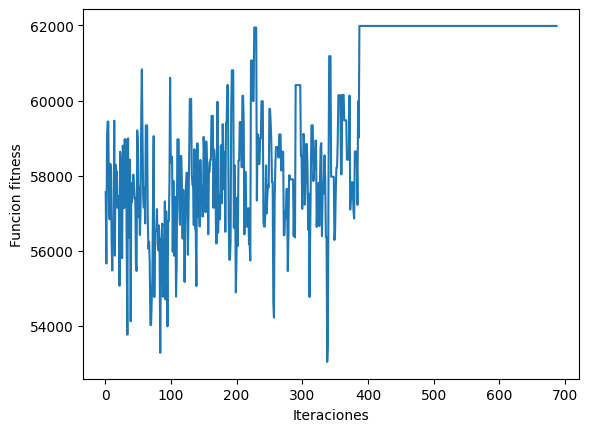
\includegraphics[width=\textwidth]{include/parada/300/f.png}
			\caption{valor: $300$}
		\end{subfigure}
		\caption{Pruebas para el criterio de parada. Evolución de la solución evaluada.}
	\end{figure}
	
	\begin{figure}[H]
		\centering
		\begin{subfigure}{0.24\textwidth}
			\centering
			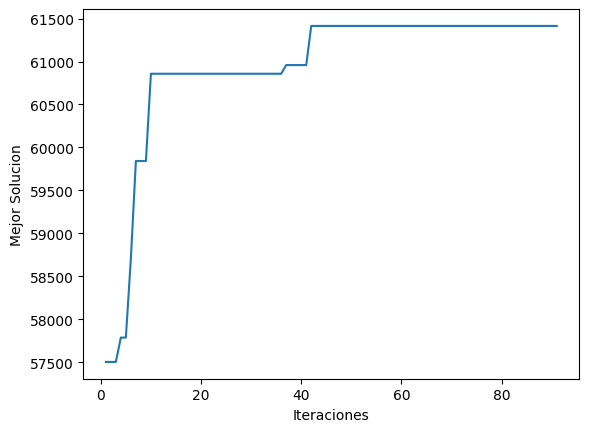
\includegraphics[width=\textwidth]{include/parada/50/f_ast.png}
			\caption{valor: $50$}
		\end{subfigure}
		\hfill
		\begin{subfigure}{0.24\textwidth}
			\centering
			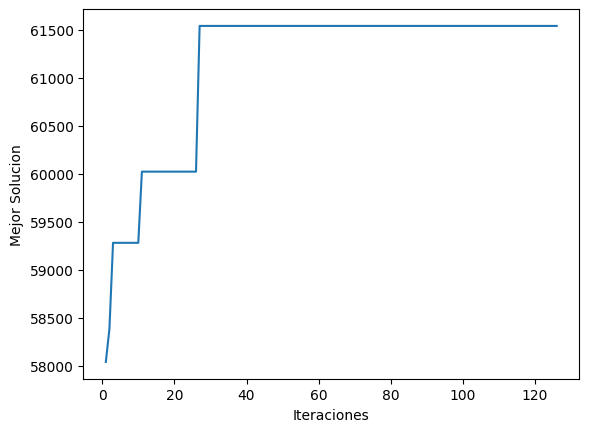
\includegraphics[width=\textwidth]{include/parada/100/f_ast.png}
			\caption{valor: $100$}
		\end{subfigure}
		\hfill
		\begin{subfigure}{0.24\textwidth}
			\centering
			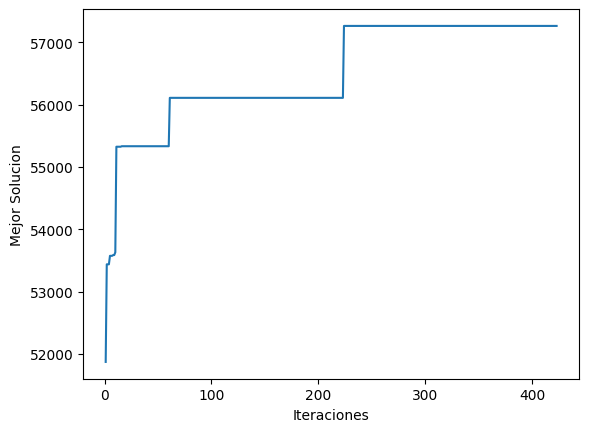
\includegraphics[width=\textwidth]{include/parada/200/f_ast.png}
			\caption{valor: $200$}
		\end{subfigure}
		\hfill
		\begin{subfigure}{0.24\textwidth}
			\centering
			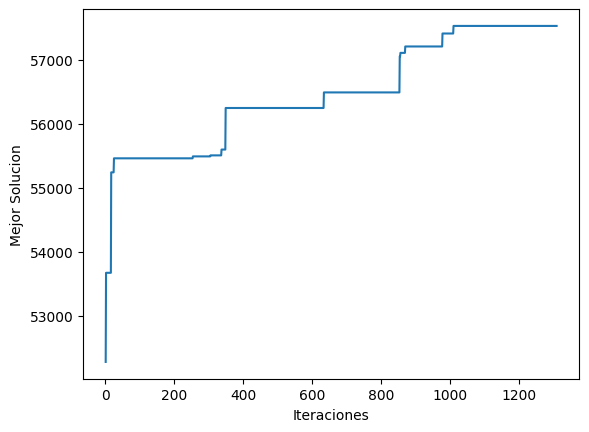
\includegraphics[width=\textwidth]{include/parada/300/f_ast.png}
			\caption{valor: $300$}
		\end{subfigure}
		\caption{Pruebas para el criterio de parada. Evolución de la mejor solución hallada.}
	\end{figure}

	\begin{figure}[H]
		\centering
		\begin{subfigure}{0.24\textwidth}
			\centering
			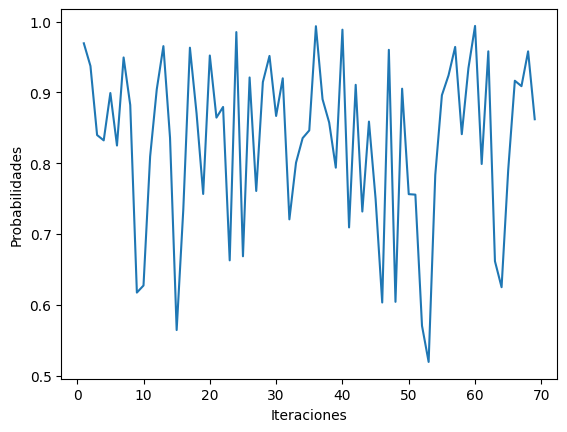
\includegraphics[width=\textwidth]{include/parada/50/prob.png}
			\caption{valor: $50$}
		\end{subfigure}
		\hfill
		\begin{subfigure}{0.24\textwidth}
			\centering
			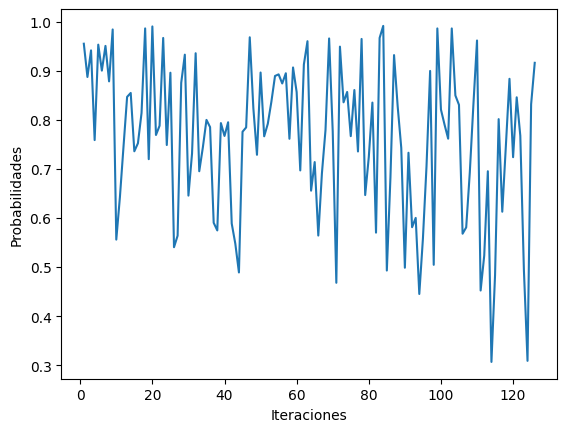
\includegraphics[width=\textwidth]{include/parada/100/prob.png}
			\caption{valor: $100$}
		\end{subfigure}
		\hfill
		\begin{subfigure}{0.24\textwidth}
			\centering
			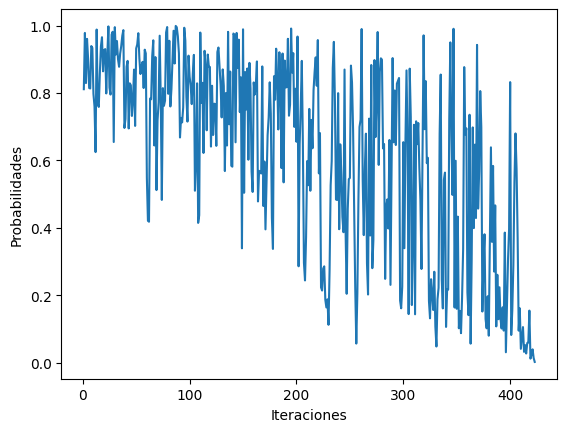
\includegraphics[width=\textwidth]{include/parada/200/prob.png}
			\caption{valor: $200$}
		\end{subfigure}
		\hfill
		\begin{subfigure}{0.24\textwidth}
			\centering
			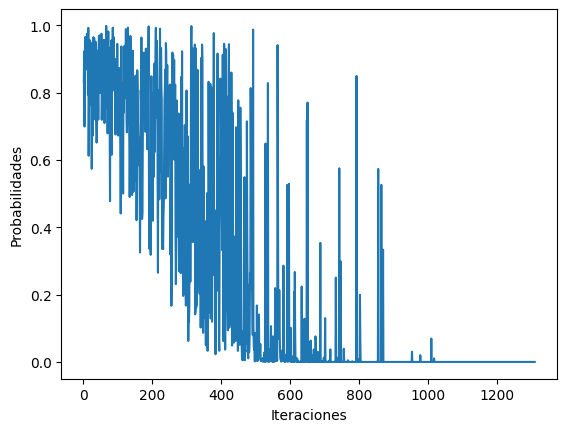
\includegraphics[width=\textwidth]{include/parada/300/prob.png}
			\caption{valor: $300$}
		\end{subfigure}
		\caption{Pruebas para el criterio de parada. Evolución de la probabilidad de moverse a soluciones peores.}
	\end{figure}
	
	Con los resultados de estas pruebas piloto se decide fijar el número de iteraciones sin cambio necesarias para que el algoritmo considere haber alcanzado un óptimo global $300$.
	
	
	
	\subsubsection{Implementación}
	El proceso de recocido simulado genera $N$ iteraciones de la simulación, modificando algunos de los valores en cada iteración.\\
	
	Para implementar en python el recocido simulado, hemos definido el método \texttt{recocido} \texttt{\_simulado}, que toma como parámetro un estado inicial, con las variables de  	decisión inicializadas. A continuación, se inicializan las variables L, Temperatura Inicial, Temperatura final, $\alpha$, Temperatura Final, el contador de iteraciones totales y el contador de pasos para cambiar la temperatura. \\

	\begin{python}
def recocido_simulado(initial_state):
	
	# HIPERPARAMETERS
	alpha = 0.95 #Ritmo de decrecimiento de la temperatura
	initial_temp = 7500
	max_it_sin_cambio = 300
	max_L = 10
	
	it_sin_cambio = 0 # Contador de iteraciones sin cambio
	L = 0 #Contador del paso
	iteraciones = 1 #Contador de iteraciones
	\end{python}

	En la primera iteracion, damos a la variable \texttt{current\_state}, que va a ir guardando el estado donde nos encontramos, el valor del estado inicial.
	Generamos los beneficios utilizando el método \texttt{get\_benef}, que ejecuta la simulación desarrollada en el primer apartado, y los guardamos en la clave
	"benef" del current\_state. Igualamos la variable \texttt{best\_state} al current\_state.\\

	\begin{python}
	# Primera iteracion
	current_temp = initial_temp
	current_state = initial_state
	current_state["benef"] = get_benef(current_state)
	best_state = current_state
	\end{python}			

	Una vez finalizada esta primera iteración, entramos en un bucle que terminará cuando la temperatura alcance el valor mínimo. Este criterio de parada es uno de los más utilizados \cite{tfm}, si bien es cierto que existen otros.\\

	\begin{python}	
while it_sin_cambio < max_it_sin_cambio:
	# Comprobar si el vecino es mejor
	neighbor = get_neighbor(current_state)
	neighbor["benef"] = get_benef(neighbor)

	benef_diff = neighbor["benef"] - current_state["benef"]
	prob = math.exp(-abs(benef_diff) / current_temp)

	# Si es mejor, aceptamos vecino
	# Si es peor, aceptamos si p>u
	if benef_diff > 0 or random.uniform(0, 1) < prob:
		current_state = neighbor
	\end{python}	

	Al entrar en el bucle, utilizamos el método \texttt{get\_neighbors} para obtener una solucion del entorno del estado actual, y de nuevo utilizando el método \texttt{get\_benef}, obtenemos el beneficio que genera el vecino, y igualamos \texttt{prob} al valor de la probabilidad siguiendo la distribución de Boltzmann para la temperatura actual. \\
	
	Si la solución es mejor, la variable \texttt{current\_state} pasa a ser el estado del vecino.
	Si la solución es peor, generamos una probabilidad aleatoria utilizando el generador \texttt{random.uniform}. Si su valor es mayor que la probabilidad inicializada previamente,
	nos quedamos con el \texttt{current\_state} actual. Si es menor, actualizamos current\_state al valor del vecino.\\

	\begin{python}	
def get_benef(state):
  		return simul_main(state["periodicidad"],
  		                  state["nivel_1"], state["nivel_2"])

def get_neighbor(state):
	"""Devuelve vecinos en un radio 1"""
	new_periodicidad = state["periodicidad"] +  np.random.uniform(-1,1)
	new_nivel_1 = state["nivel_1"] +  random.randint(-3,3)
	new_nivel_2 = state["nivel_2"] +  random.randint(-3,3)

	neighbor = {'periodicidad':new_periodicidad ,  
					'nivel_1': new_nivel_1,
					'nivel_2': new_nivel_2 }

	return neighbor
	\end{python}		

	Dentro del mismo bucle, una vez se ha hecho el cambio de estado, se pasan por dos condicionales. En primer lugar, si el contador de pasos ha llegado al valor L, que recordamos es 10, entonces
	actualizamos la temperatura. En segundo lugar, si la solución almacenada en \texttt{best\_state} es peor que la del estado actual, actualizamos \texttt{best\_state}.
	Esta modificación la hemos añadido para evitar que el algoritmo haya pasado en las primeras iteraciones por el mínimo global, y al rectificar haya terminado en un mínimo local.\\

	\begin{python}
	# Bajamos temperatura
	if L==max_L:
		current_temp = current_temp * alpha
		L=0
	
	iteraciones += 1
	L += 1
	it_sin_cambio +=1 
	
	if best_state["benef"] < current_state["benef"]:
		best_state = current_state		it_sin_cambio = 0
	\end{python}

	Cuando se alcanza la temperatura mínima, el algoritmo se detiene y el método devuelve el \texttt{best\_state}.

	
	\subsubsection{Resultados}
	Los mejores resultados se han obtenido al inicializar los hiperparámetros identificados previamente a los siguientes valores:
	\begin{itemize}
		\item La temperatura inicial es de $7\hspace{1mm}500$ grados. Probando con valores menores, como $9\hspace{1mm}000$, no se alcanzaba el mínimo global.
		\item La temperatura final es de $0.1$ grados
		\item $\alpha$ es $0.95$, siguiendo las recomendaciones (Hajek, 1988).
		\item El valor de L es de $10$ pasos
		\item La distancia de las soluciones exploradas es $1$ para la periodicidad y $3$ para el nivel de inventario.
		\item El criterio de parada son $300$ iteraciones sin cambios.
	\end{itemize}
	Para estos hiperparámetros, hemos conseguido un beneficio de $62\hspace{1mm}006.913€$, siendo $x€$ unidades mayor que el del estado inicial. \\
	%{'periodicidad': 165.629957928881, 'nivel_1': 1070, 'nivel_2': 1470, 'benef': 62006.91302597619}
	
	Cabe destacar que, al inspeccionar los \textit{logs} que hemos impreso, el mínimo global se alcanza $150$ iteraciones antes del final. Hemos probado a optimizar este resultado alterando el valor de $L$ y la temperatura final, pero ninguna de las dos modificaciones ha dado resultados satisfactorios. \\
	
	
	
	% - GRAFICAS Y COMENTARLAS --------------------------------------------------------------------------------
	
	Tras la optimización de la simulación mediante el recocido simulado obtenemos las gráficas de rendimiento de la Figura \ref{result-graphs}, que representan la evolución de los valores de diferentes parámetros y funciones durante la simulación.\\
		
	En ellas se puede observar como afecta el descenso de la temperatura a la probabilidad de moverse a soluciones peores, ya que con mayor temperatura, mayor es la probabilidad de moverse a un estado peor y con temperatura más cercanas a cero, esa probabilidad es prácticamente nula.\\
	
	También se observa esta evolución en las gráficas de la función $f$ y $f*$, donde vemos que en las primeras iteraciones, la solución evaluada es más variable mientras que en las últimas iteraciones ambas gráficas se asemejan.\\
	
	Es también interesante señalar la variación de los factores de evolución, que varían de manera inversamente proporcional entre sí, ya que en general, al aumentar el valor de uno, disminuye el del otro.
	
	\begin{figure}[H]
		\centering
		\begin{subfigure}{.45\textwidth}
			\centering
			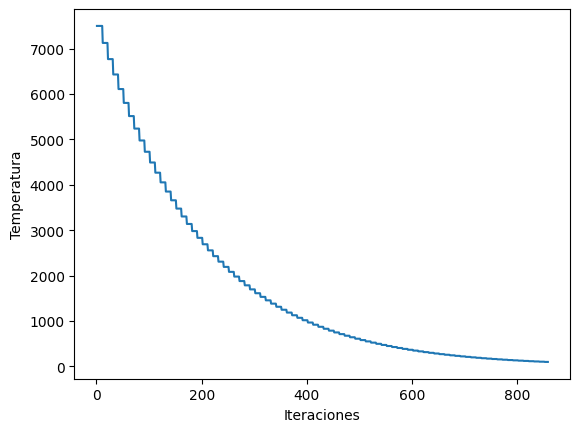
\includegraphics[width=\textwidth]{include/ultima_ejec/temp.png}
			\caption{Evolución de la temperatura. }
		\end{subfigure}
		\hfill
		\begin{subfigure}{.45\textwidth}
			\centering
			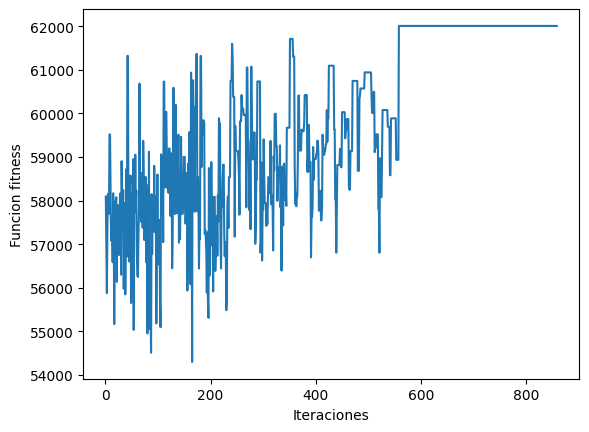
\includegraphics[width=\textwidth]{include/ultima_ejec/f.png}
			\caption{Evolución de la solución evaluada. }
		\end{subfigure}
		\hfill
		\begin{subfigure}{.45\textwidth}
			\centering
			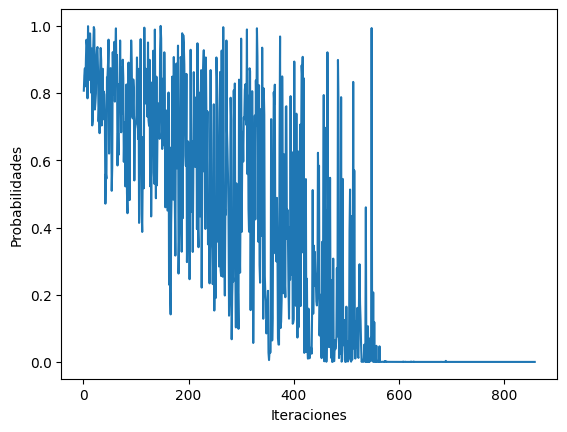
\includegraphics[width=\textwidth]{include/ultima_ejec/prob.png}
			\caption{Evolución de la probabilidad de moverse a soluciones peores. }
		\end{subfigure}
		\hfill
		\begin{subfigure}{.45\textwidth}
			\centering
			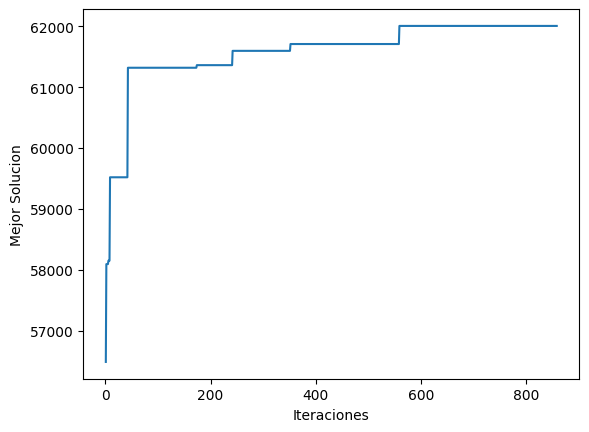
\includegraphics[width=\textwidth]{include/ultima_ejec/f_ast.png}
			\caption{Evolución de la mejor solución hallada. }
		\end{subfigure}
		\hfill
		\begin{subfigure}{.45\textwidth}
			\centering
			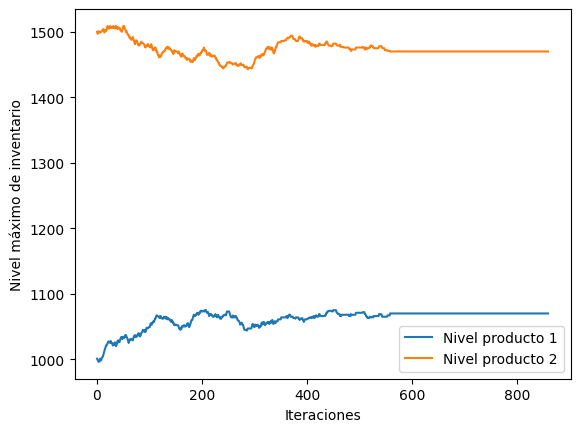
\includegraphics[width=\textwidth]{include/ultima_ejec/niv_inv.png}
			\caption{Evolución de los niveles de inventario. }
		\end{subfigure}
		\hfill
		\begin{subfigure}{.45\textwidth}
			\centering
			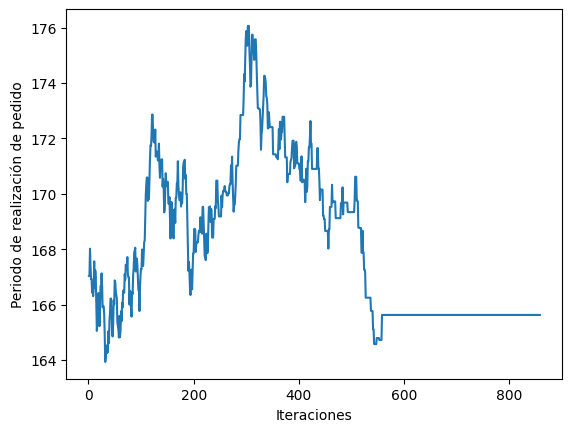
\includegraphics[width=\textwidth]{include/ultima_ejec/periodo.png}
			\caption{Evolución del periodo de realización de pedido. }
		\end{subfigure}
		\caption{Gráficas de rendimiento de la simulación con los parámetros elegidos.}
		\label{result-graphs}
	\end{figure}
	
	\section{Conclusiones}
	En este ejercicio, hemos simulado un problema sencillo de almacén durante 5 meses que estaba caracterizado por una política de pedidos periódica, y dos tipos de producto disponibles. Hemos aprendido la diferencia entre las rutinas que necesita una política de pedidos periódica y aperiódica. También hemos podido observar el aumento de complejidad al aumentar el número de productos,
	que, aunque en este caso sigue siendo un número pequeño, nos permite comprender la complejidad que tendría trabajar con la simulación de un almacén real. \\
	
	En segunda lugar, hemos podido implementar la metaheurística de recocido simulado para optimizar la 
	simulación. Cabe destacar la importancia de la selección de hiperparametros, que ha sido probablemente la tarea más compleja de todo el proyecto. Esto se debe en efecto a la naturaleza aleatoria del problema, 
	que conduce a una elección empírica de los mismos. En concreto, ha sido interesante observar como los valores de la temperatura condicionaban la convergencia del algorimto, y la importancia de elegir una temperatura lo suficientemente elevada para que este tenga una 
	fase exploratoria. Sería interesante comparar la solución obtenida con esta metaheurística con otros tipos, como por ejemplo los algoritmos genéticos.
	\newpage
	\section*{Bibliografía}
	\addcontentsline{toc}{section}{Bibliografía}
	\bibliography{include/references}
	\bibliographystyle{IEEEtran}
	
\end{document}